\section{Trivia Game}

The first modality of the game is a trivia-type game, that will use Romie, the robot in
WebLab-Deusto and its labyrinth to create an experience for learning general knowledge. Moreover,
since the trivia questions will be configurable, so that the game can be adapted.

\subsection{Software and Hardware Requirements}

This software will have tight requirements in terms of user-friendliness, communication stability
and security, since it must be developed using as far as possible current hardware and be easy to
use by young students. Moreover, since it will be presented in crowded events, it must support high
load and availability.

Furthermore, due to the requirements of the project, it must be integrated with the WebLab-Deusto
platform and must be deployable in that environment. Thus, the requirements specification will be
as it follows:

\subsubsection{Software requirements:}

\begin{itemize}
	\item The software must be able to communicate with the robot.
	\item The software must be able to send control commands to the robot.
	\item The software must be able to receive command results from the robot.
	\item The software must be integrated in the WebLab-Deusto platform as a new experiment.
	\item The software must have an easy to use user interface based on human-computer interaction
	principles.
	\item The software must be stable enough to support tens of accesses per hour.
	\item The software must provide enough questions so that the user never finishes with them and
	can be randomly selected.
	\item The game must increase difficulty as the user gets more points.
	\item The game must finish in less than 15 minutes.
	\item A ranking must be provided after finishing the game for the user to know its ranking.
\end{itemize}

\subsubsection{Hardware requirements:}

\begin{itemize}
	\item The hardware must be placed in WebLab-Deusto.
	\item The robot must never get blocked, so in the case of an incident it must be automatically
	recovered.
	\item The cameras must be accessible from the Internet.
	\item The robot must be controlled via Bluetooth.
	\item The robot must never run out of power.
	\item The robot must be able to read all the \acrshort{rfid} tags with at least 99~\% accuracy.
	\item The robot must use the current labyrinth in WebLab-Deusto.
	\item No new hardware can be added to the current WebLab server (Plunder).
\end{itemize}

\subsection{Design Specification}

Taking into account the previous requirements, it has been decided to do a small hardware redesign
and a complete software design for the project. We will now see the hardware and software design
specifications.

\subsubsection{Hardware Specification}

Current robot is deployed with a simple \acrshort{rfid} (\acrlong{rfid}) reader (model ID-12) not
capable of reading further than 120~mm~\cite{rfid}, which has shown some issues when reading the
\acrshort{rfid} tags. For that reason, it has been decided to use a new module, the model ID-20LA
(figure~\ref{fig:rfid}). This will give the robot a much higher reliability when reading
\acrshort{rfid} tags, and the range of the new sensor is 180~mm~\cite{rfid}.

\begin{figure}[!htbp]
	\centering
	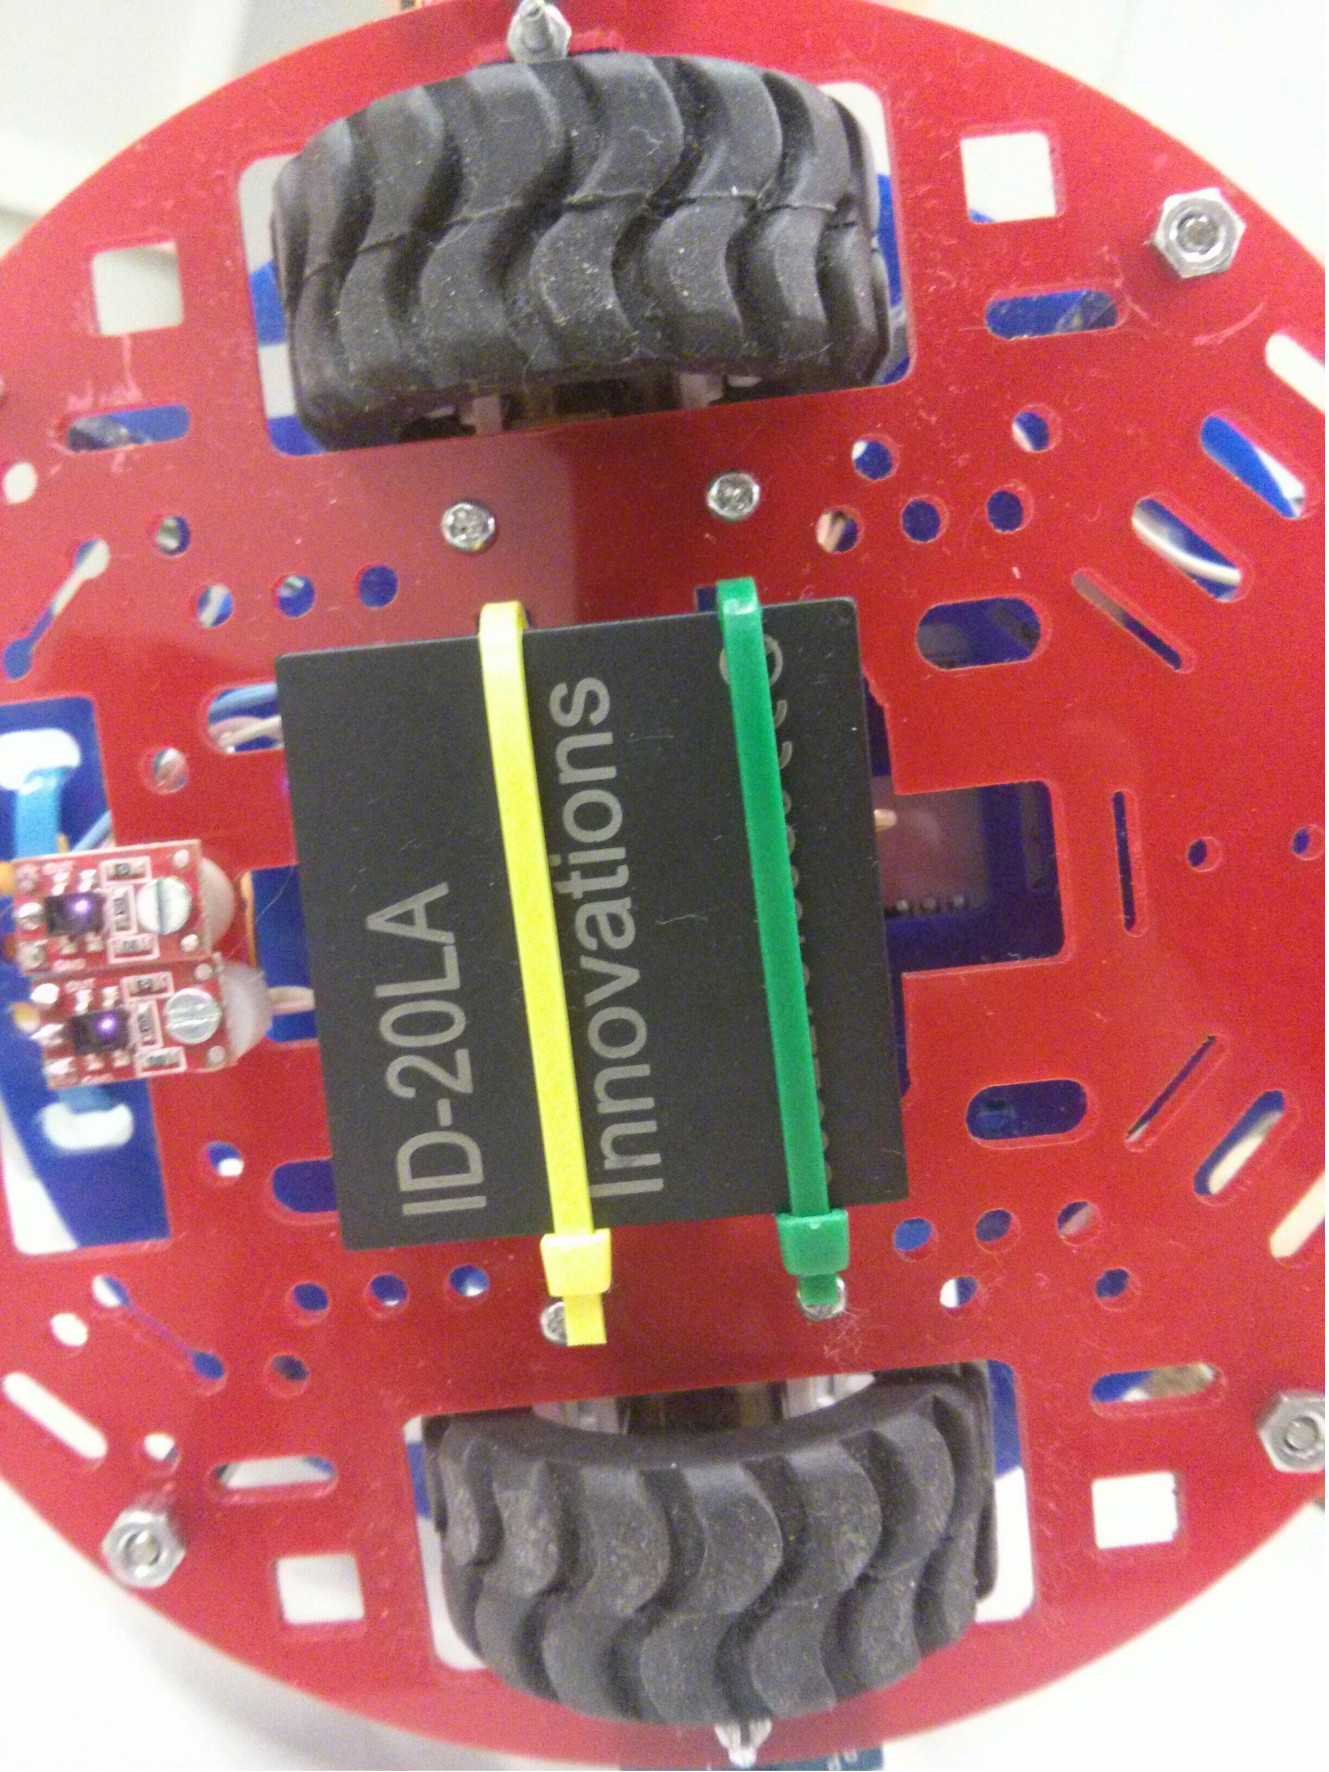
\includegraphics[width=0.3\textheight, angle=-90]{fig/rfid}
	\caption{ID-20LA \acrshort{rfid} reader.}
	\label{fig:rfid}
\end{figure}

On the other hand, there is currently an issue with the availability of the robot. It is powered
with a 2Ah \acrshort{lipo} battery, and is recharged when needed. This has a big issue, since as we
have seen, in high load conditions would not meet the required availability, and furthermore, in
weekends or holidays, we will not be able to change and recharge the battery, so it has been decided
to deploy a cable installation from the roof of the ceiling of the laboratory, and the design of the
robot has been adapted so that the cables do not get stuck in the labyrinth.

The rest of the robot will be used as it is, since it provides with the needed capabilities for the
needs of the project: It has a wall sensor capable of avoiding crashes with walls, infrared sensors
to detect the lines in the ground, motors and wheels capable of moving the robot, Bluetooth
connection to communicate with it and Arduino microcontroller, to install the needed firmware
(figure~\ref{fig:bluetooth}).

\begin{figure}[!htbp]
	\centering
	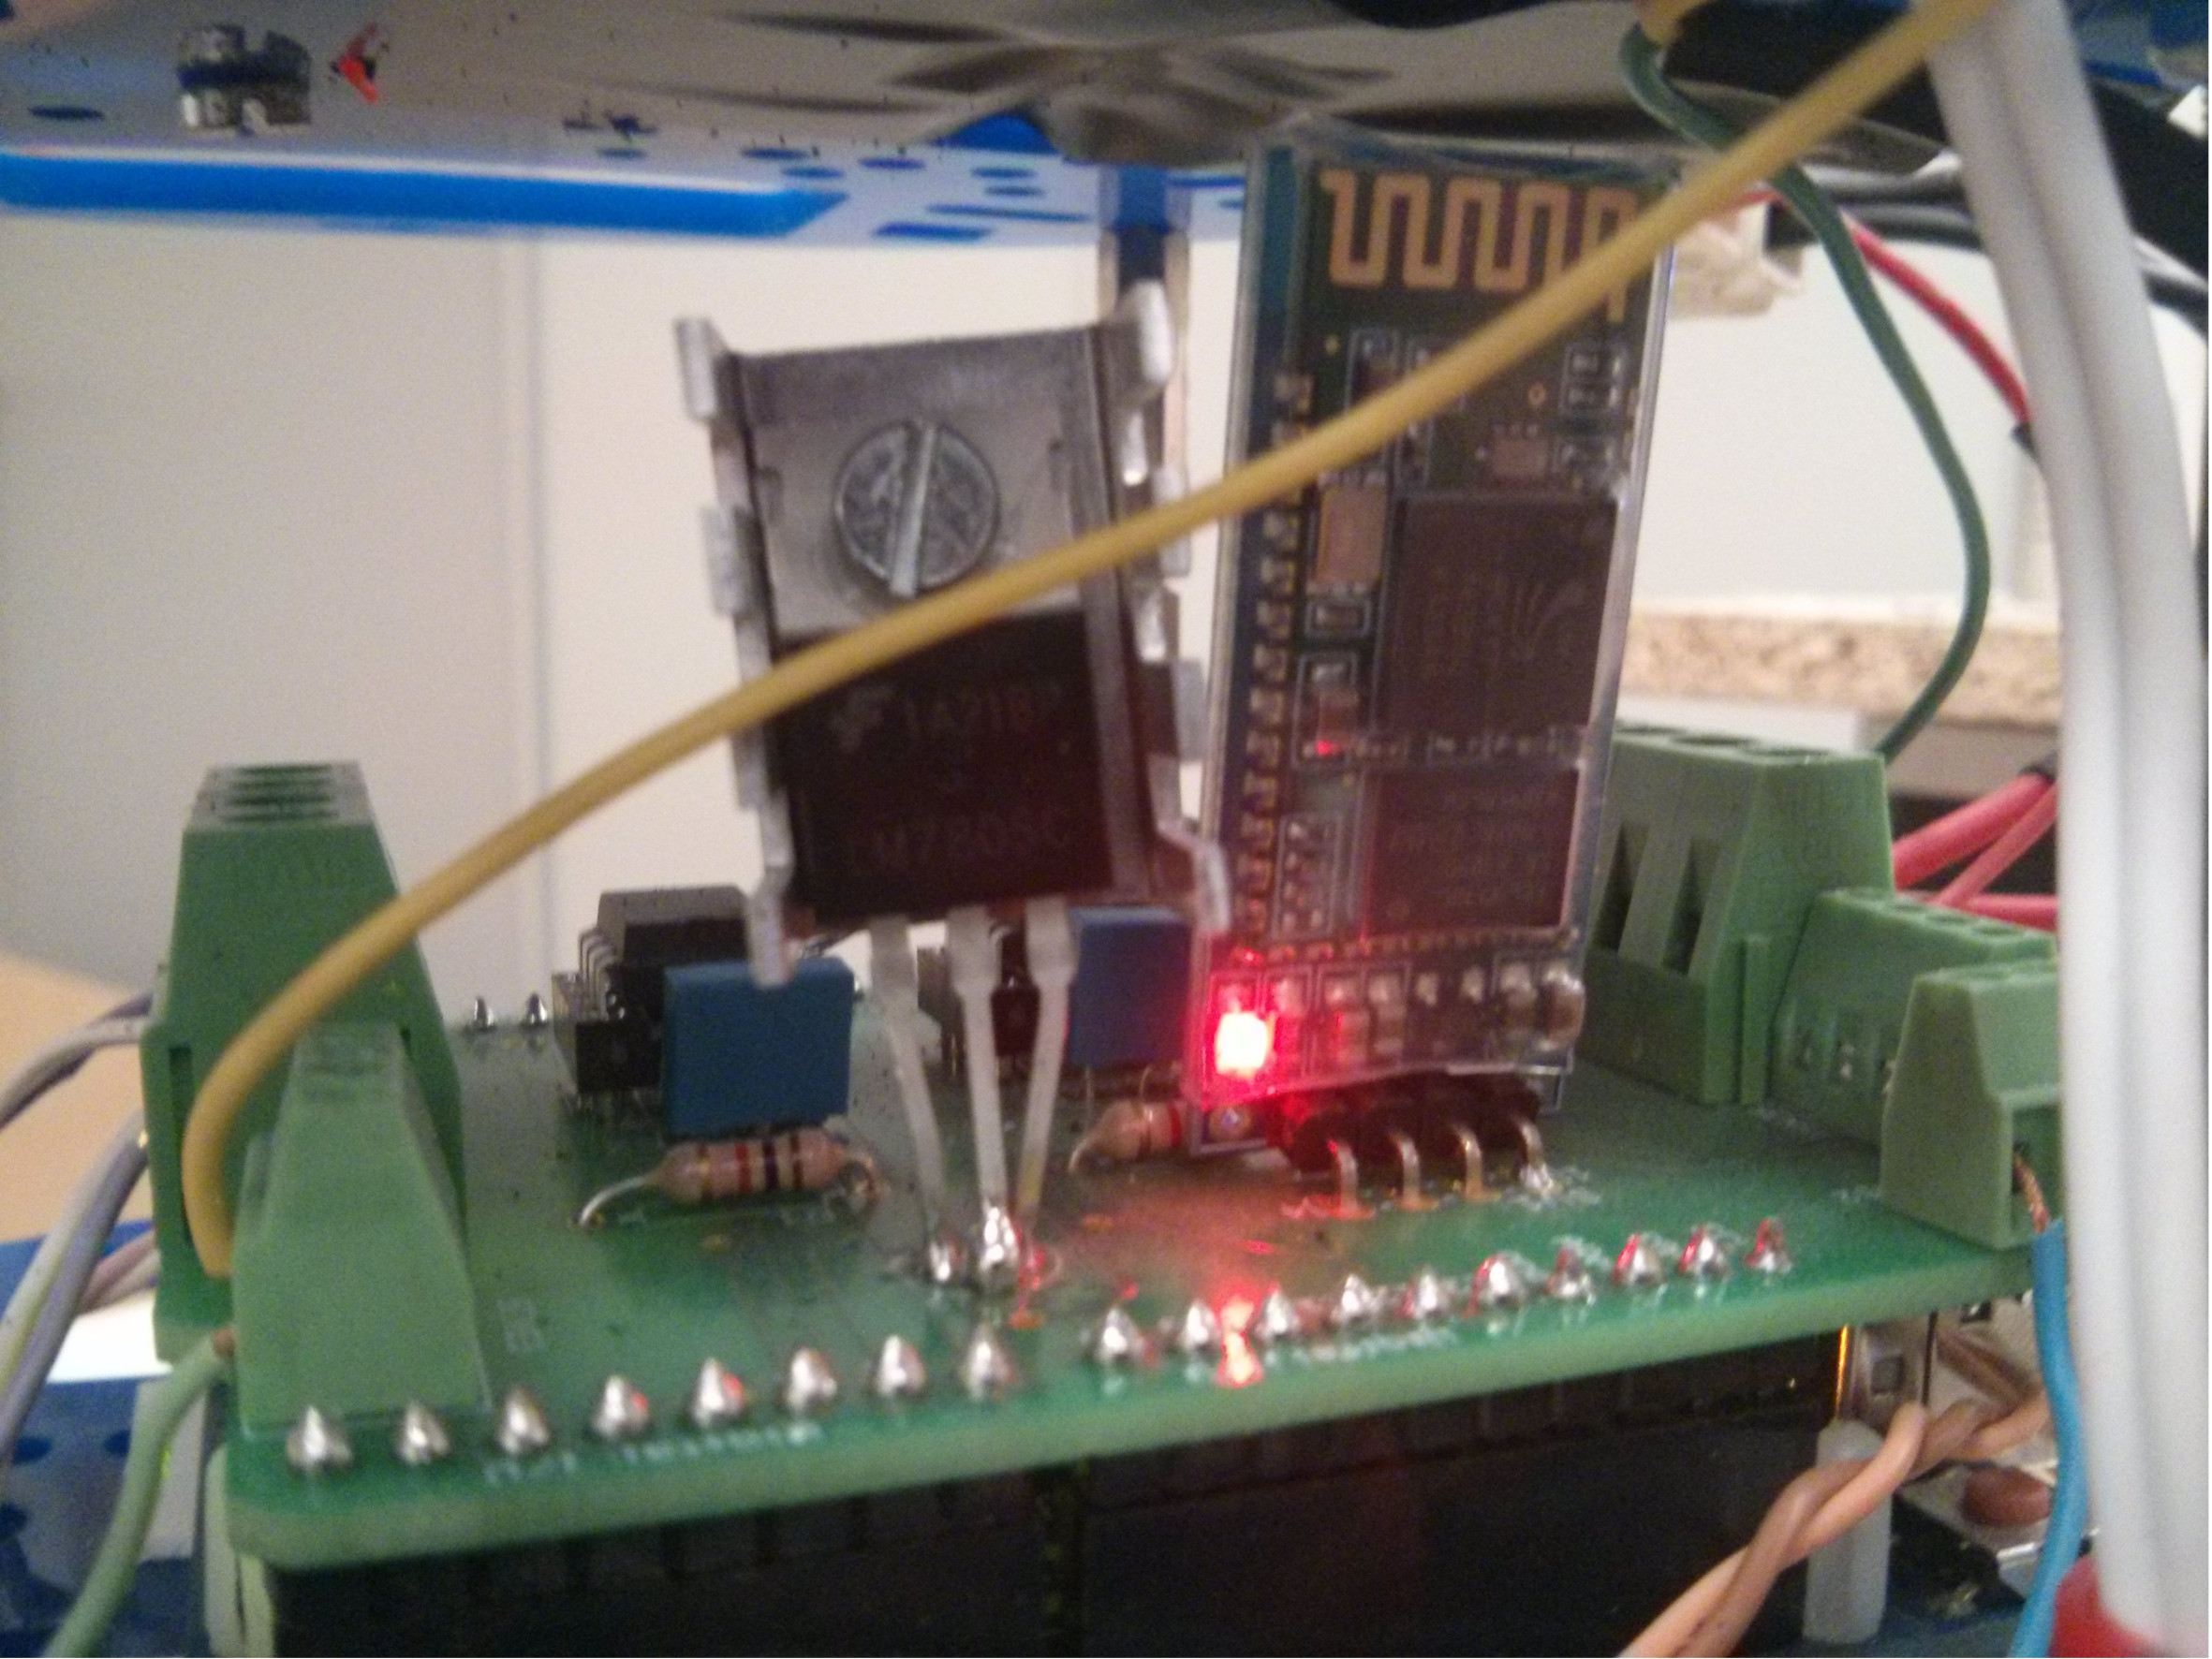
\includegraphics[width=0.65\textwidth]{fig/bluetooth}
	\caption{Bluetooth module on top of the Arduino shield.}
	\label{fig:bluetooth}
\end{figure}

The robot is currently configured with a camera D-link DCS-932L that provides infrared vision if the
light is shut down and normal vision if not, and it can be accessed from Wi-Fi and
Ethernet~\cite{camera}. In this case we will use it via Wi-Fi, since the robot will be moving around
a big space.

\subsubsection{Software Specification}

The software in for this implementation will be divided modularly, thinking on scalability and
code reuse. The application must be built on top of WebLab-Deusto, so we will use as much as
possible the provided \acrshort{api}s. Moreover, and due to deployment needs, the software will be
divided between the robot, an intermediate server and WebLab software.

The robot will use a slightly modified version of the current firmware, since we need it not to get
blocked by any wall in case of crash and we need a more reliable implementation. That is why it has
been programmed to turn back if a hardware error occurs and collides with a wall. Nevertheless, the
external Bluetooth \acrshort{api} will be the same as the one that was already implemented at the
beginning of the project:

It will provide a ``F'' command to go forward, that will return the \acrshort{rfid} tag if it finds
one, a ``L'' command to turn left, its counterpart ``R'' command to turn right and it will also
provide the command ``S'' that will check if there is a wall in front of the robot. Nevertheless,
and even if the experiment server can check for a wall, the robot itself has been programmed to
return a ``NAK'' command if it is commanded to go forward against a wall.

The robot itself works following the lines in the labyrinth until it finds an intersection. It is
also capable of turning in those intersections, so if it is commanded to turn right, it will perform
a 90 degree turn right and face the path in its right. When the robot stops on top of a
\acrshort{rfid} tag, it will return the tags address.

The intermediate server will provide a small \acrlong{rest} (\acrshort{rest}) \acrshort{api} in a
small Python server. Its only duty will be to provide a simple interface for the robot using
\acrshort{http} instead of Bluetooth, needed due to deployment constraints. We can see an example of
the \acrshort{api} usage with Python in algorithm~\ref{alg:romie_rasp}.

\begin{center}
\begin{minipage}{.9\textwidth}
\singlespace
\begin{pyglist}[language=python, caption={Romie \acrshort{rest} \acrshort{api} example.},
	label={alg:romie_rasp}, listingname={Algorithm}, numbers=left]
import urllib2

# Let's go forward and get RFID tag if exists
tag = urllib2.urlopen('http://192.168.0.190:8000/f', timeout = 60).read()

# Let's turn left
result = urllib2.urlopen('http://192.168.0.190:8000/l', timeout = 60).read()

# Let's turn right
result = urllib2.urlopen('http://192.168.0.190:8000/r', timeout = 60).read()

# Let's check if we have a wall in front of us
result = urllib2.urlopen('http://192.168.0.190:8000/s', timeout = 60).read()
\end{pyglist}
\end{minipage}
\end{center}

Then, the experiment server required by the WebLab-Deusto architecture, will provide a WebLab
command \acrshort{api}, that will be callable by the client of the experiment. This server will be
developed in Python because the WebLab server libraries are better intended for this language. The
data for the ranking will be stored in a SQLite 3 database. This database provides all the needed
\acrshort{acid} constraints (\acrlong{acid}) with a small \acrshort{sql} (\acrlong{sql}) a
\acrlong{rdbms} (\acrshort{rdbms})~\cite{sqlite}.

The experiment server \acrshort{api} will have all the needed commands to use the experiment. For
the ones that need data being sent to the server, \acrshort{json} has been used (\acrlong{json}). It
is preferred over \acrshort{xml} (\acrlong{xml}) due to the higher compatibility of \acrshort{json}
and the more data-orientation of this \acrlong{rfc} or \acrshort{rfc}. This provides lower
overhead~\cite{xml_vs_json}.

\begin{itemize}
	\item ``\textbf{F}'', ``\textbf{L}'' and ``\textbf{R}'' commands, to move forward and turn left
	and right. The ``S'' command is not provided since the experiment does not require it and the
	robot will not drive towards a wall. The ``\textbf{F}'' will return a random question based on
	the current user's points.

	\item ``\textbf{CHECK\_REGISTER}'' command, to check if the user has been registered in the
	experiment before and decide if the experiment should show the registration form.

	\item ``\textbf{REGISTER}'' command, to send the registration data to the server and insert it
	into the SQLite database.

	\item ``\textbf{ANSWER}'' command, to send the answer given by the user to a question. It will
	return the new date for finishing the experiment and the new points for the user. These will not
	change if the answer was not correct.

	\item ``\textbf{FINISH}'' command, to finish the experiment and receive the final ranking.
\end{itemize}

Finally, the client will be developed using \acrshort{html} 5 (\acrlong{html} version 5), JavaScript
(using JQuery library) and Bootstrap for a rapid development. It will use the WebLab JavaScript
library to communicate with the experiment server. This library is an asynchronous \acrshort{ajax}
(\acrlong{ajax}) library that provides a simple interface to interact with experiments. We can see
an example in algorithm~\ref{alg:weblab_lib}.

\begin{center}
\begin{minipage}{.9\textwidth}
\singlespace
\begin{pyglist}[language=javascript, caption={WebLab JavaScript library example.},
	label={alg:weblab_lib}, listingname={Algorithm}, numbers=left]
// Callback registration that will be
// called after reserving the experiment
Weblab.setOnStartInteractionCallback(start);

// Sending command to the experiment server
Weblab.sendCommand("L", function(response) {
    console.log("Good response: " + response);
}, function(response) {
    console.log("Bad response: " + response);
});
\end{pyglist}
\end{minipage}
\end{center}

TODO: Software design graphic (experiment flow chart)

\subsection{Deployment Considerations}

The deployment must be done in WebLab-Deusto, a remote laboratory environment with three custom
networks and limited physical space. In figure~\ref{fig:weblab-network} we can see the network of
WebLab-Deusto. As we can see, Plunder is the core server. It provides access to WebLab-Deusto web
environment and it provides most of the experiment servers. On the other hand, Blood is the one
working as a proxy for all the cameras in WebLab-Deusto, some of them connected by Wi-Fi and others
by Ethernet.

\begin{figure}[!htbp]
	\centering
	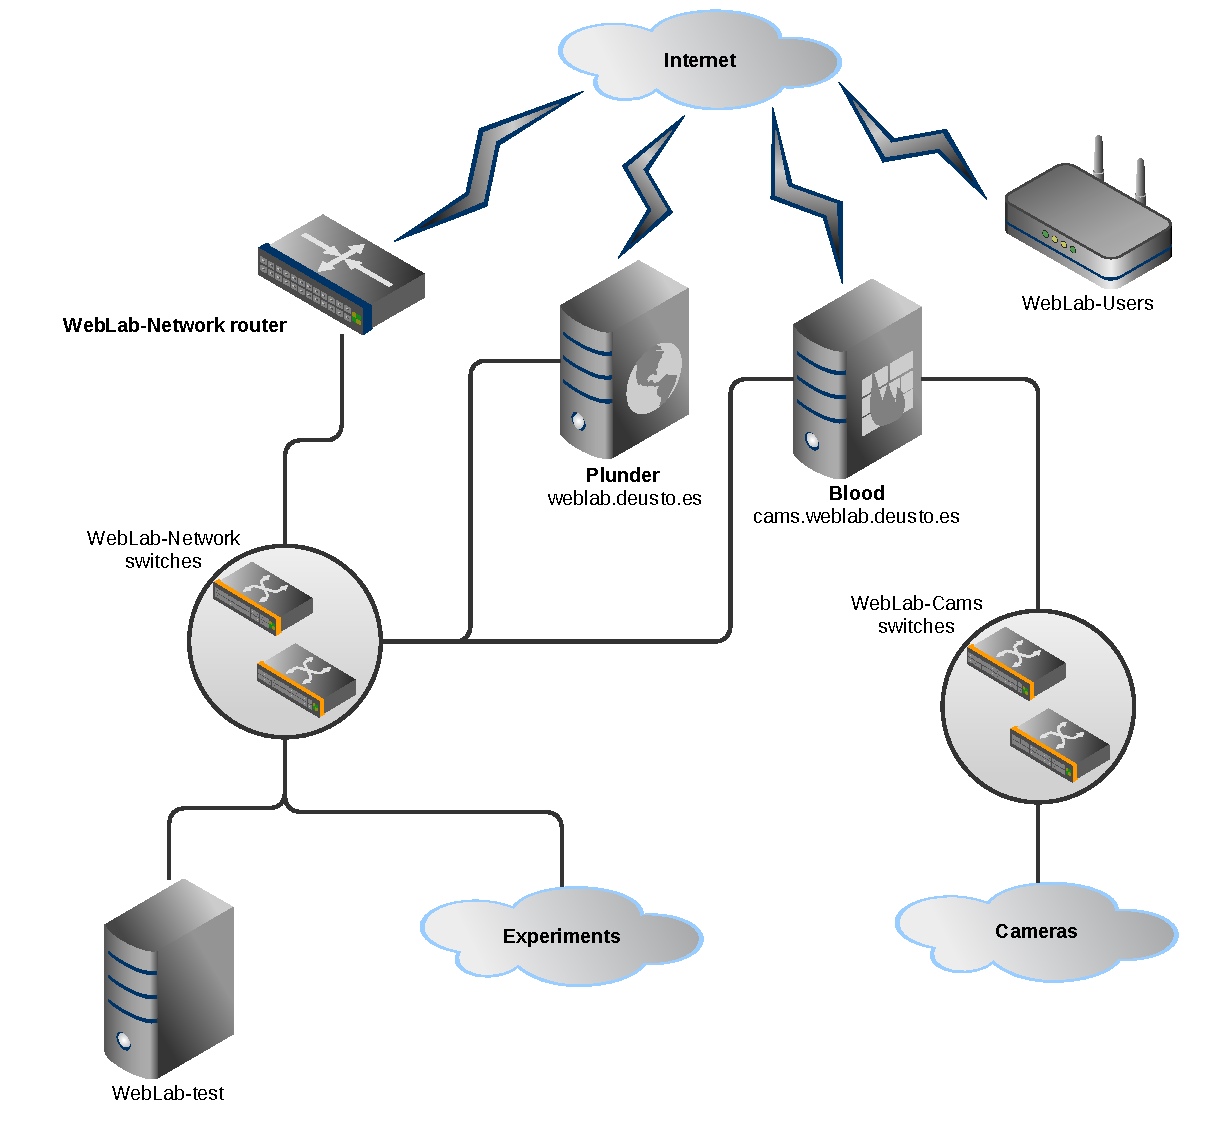
\includegraphics[width=0.9\textwidth]{fig/weblab-network}
	\caption{WebLab-Deusto network simplification.}\label{fig:weblab-network}
\end{figure}

In this case, since we need Bluetooth to connect our experiment server to the robot, and Plunder,
Blood and WebLab-test should not need new hardware, we will use a Raspberry Pi Model B
(figure~\ref{fig:rasp}) with a \acrshort{usb} (\acrlong{usb}) Bluetooth dongle to connect to the
robot and to provide a simple \acrshort{http} server with the \acrshort{rest} \acrshort{api}. This
small computer provides us with the needed hardware for such small web server, since it provides
512~MB of \acrshort{ram}, a 700~Mhz \acrshort{arm} \acrshort{cpu}, 2 \acrshort{usb} ports and an
Ethernet port. All this in a small form factor, not bigger than a usual credit card, and consuming
only 3.5~W~\cite{rasp_b}.

\begin{figure}[!htbp]
	\centering
	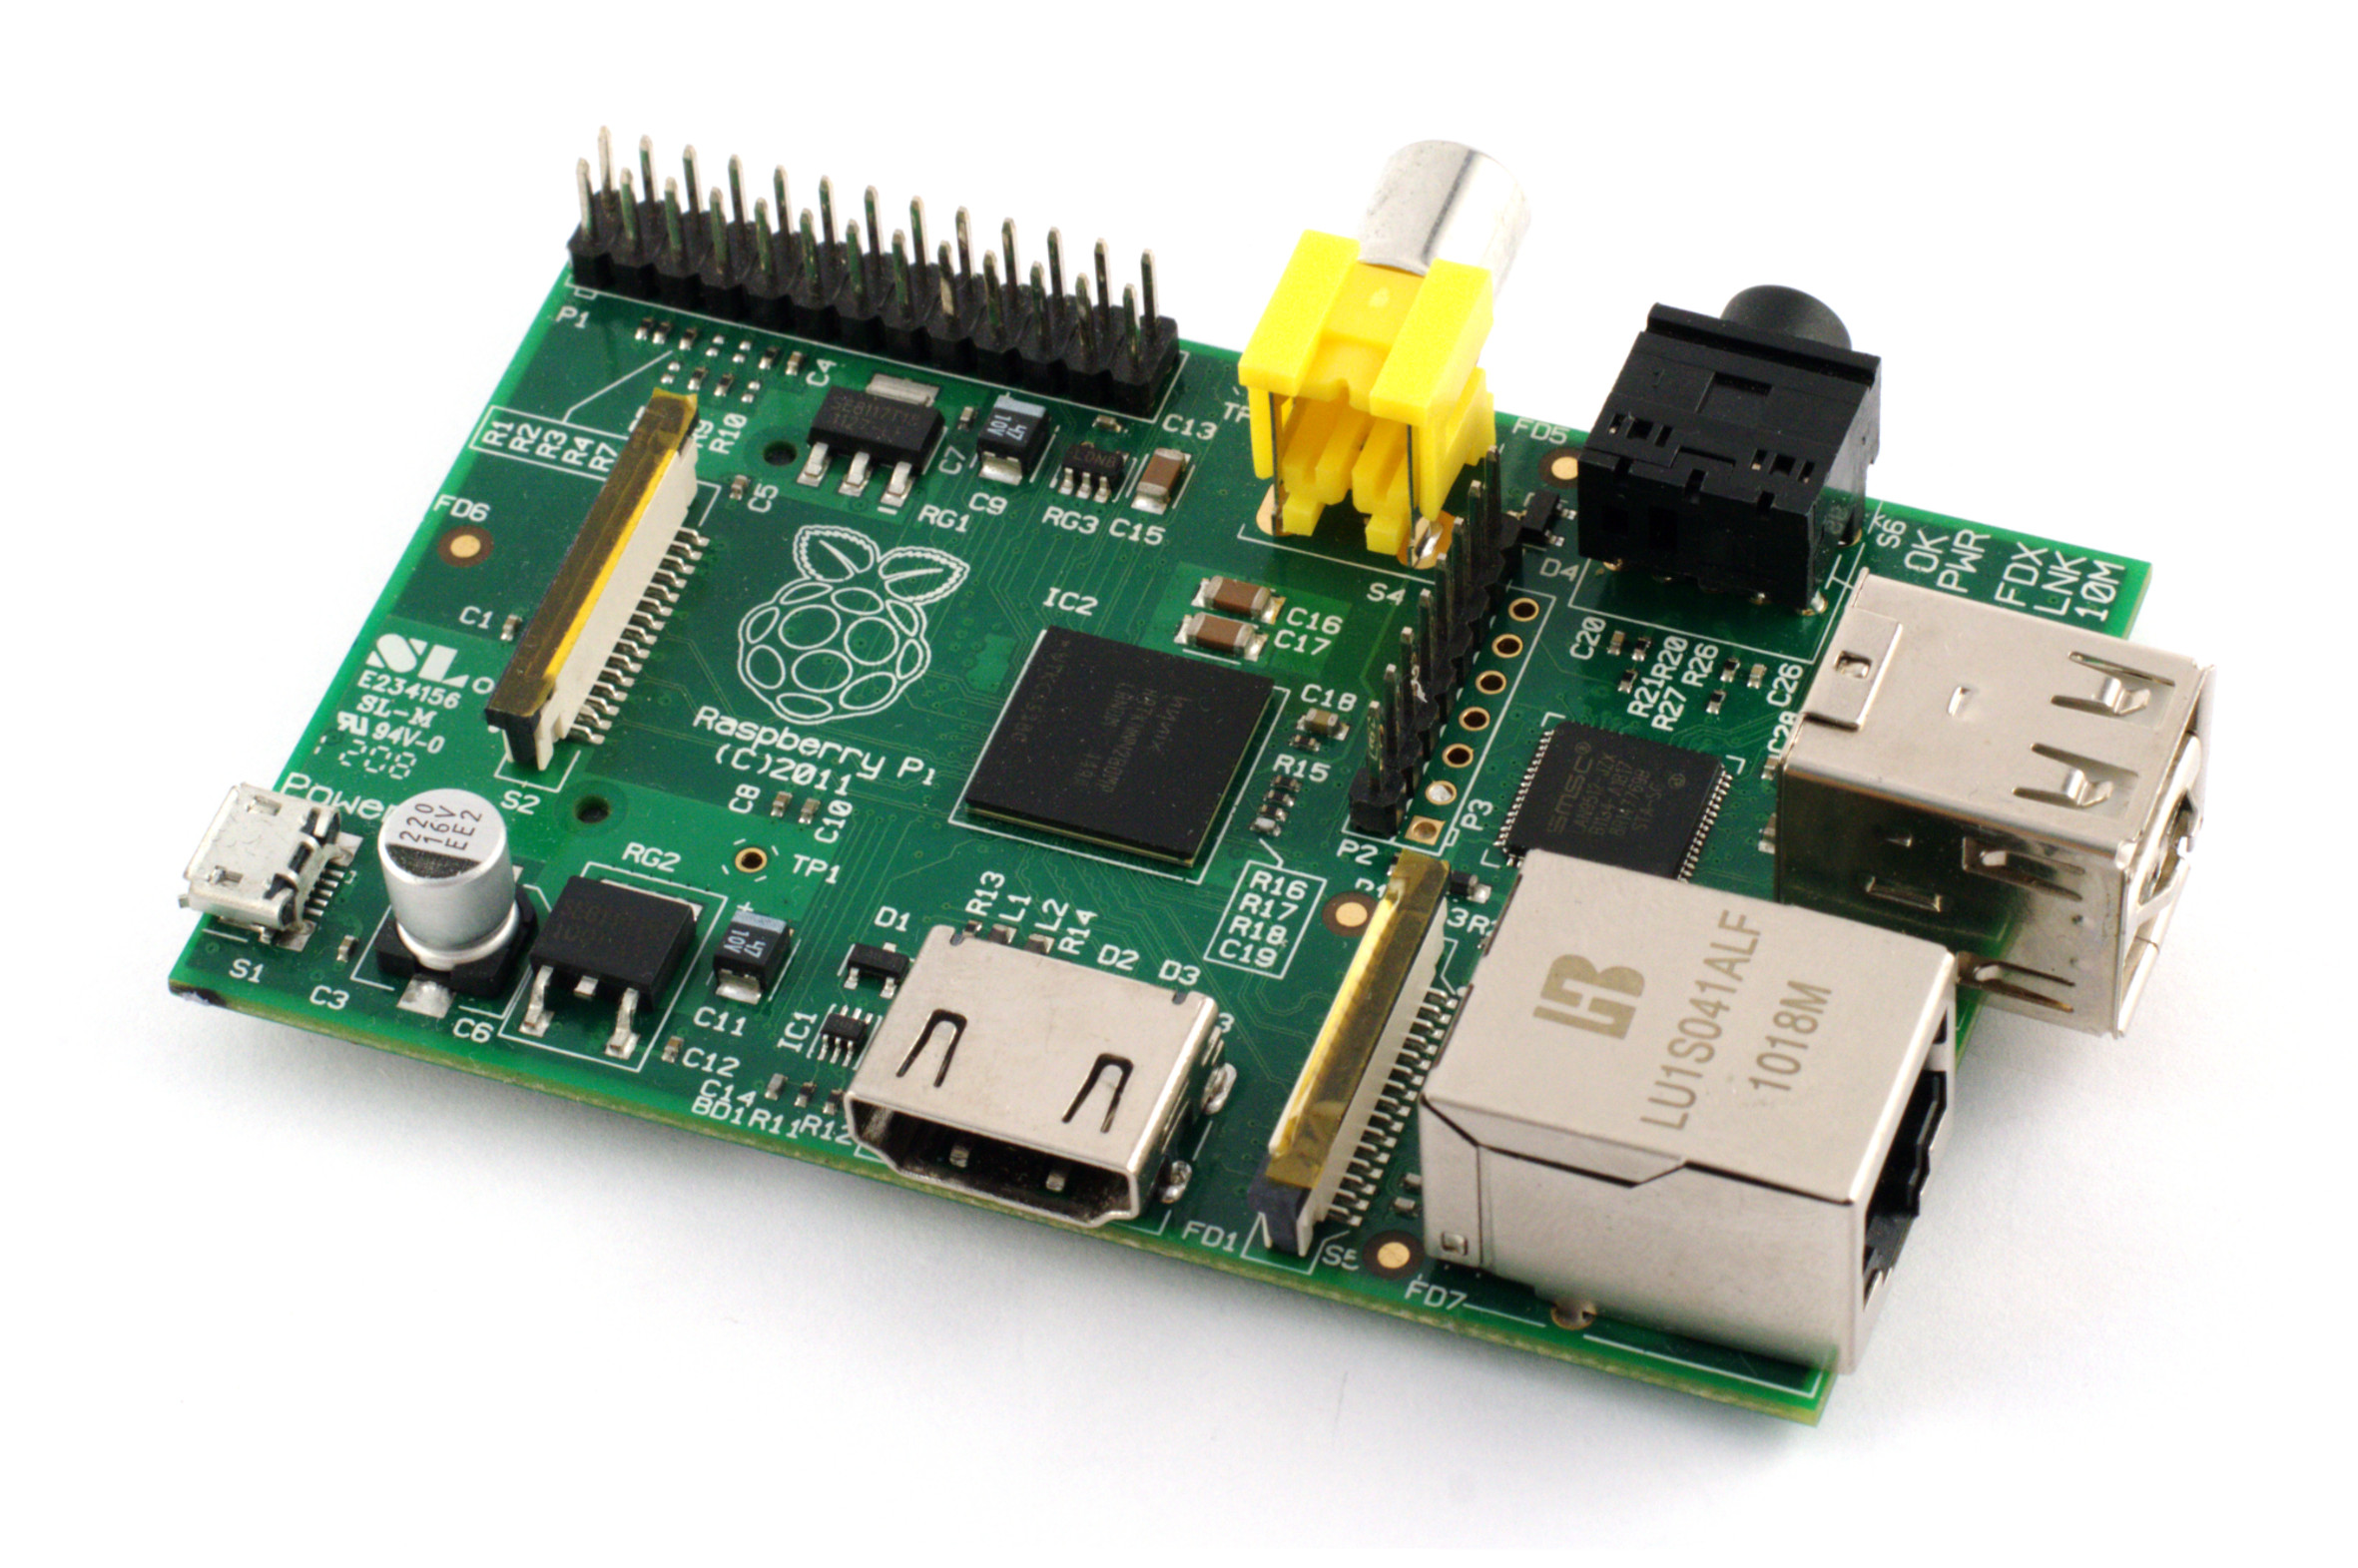
\includegraphics[width=0.7\textwidth]{fig/rasp}
	\caption{Raspberry Pi model B computer.}
	\label{fig:rasp}
\end{figure}

This small computer will be connected via Ethernet to the WebLab network, while two cameras (the top
camera and the on-board camera) will be connected via Wi-Fi to WebLab camera network, using Blood as
the \acrshort{http} proxy server.

Finally, since the server software will change many times during the development, and Plunder must
be restarted for each change if the experiment server is located there, the experiment server for
this experiment will be located in WebLab-test. This way, there will be no need to restart Plunder
each time a new change is made to the experiment, giving higher availability to WebLab-Deusto.

\subsection{Testing Plan}

The testing for this software is divided in 3 main environments. First of all, the usual manual
testing is made by the developers and by the administrators of WebLab-Deusto. This showed many bugs
that we were able to fix almost as soon as they appeared, but in any case, this is not enough
for a production environment.

After the manual testing, WebLab-Deusto has a \acrlong{ci} system connected to Travis \acrshort{ci}
in GitHub. It provides many unit tests that provide stability to the code, since we receive emails
when a commit does not pass the tests. Nevertheless, for the \acrlong{gui} or \acrshort{gui}, it is
difficult to provide unit tests.

Finally, and also as a demonstration of the potential of the project, we tested the project in an
event at the University of Deusto called ForoTech~\cite{forotech}. In this event we were be able to
test the project in a high load environment, where the robot received more than a hundred uses in a
short period of time, demonstrating the reliability and also giving us the possibility to fix some
issues.

\subsection{User Manual}

For using Romie, you must have an account in WebLab-Deusto and the appropriate permissions to use
the experiment. Once you fulfill those requirements, go to
\url{https://weblab.deusto.es/weblab/client/}. In that page (figure~\ref{fig:man:weblab}), you will
be able to insert your credentials in the login form and log in.

\begin{figure}[ht]
	\centering
	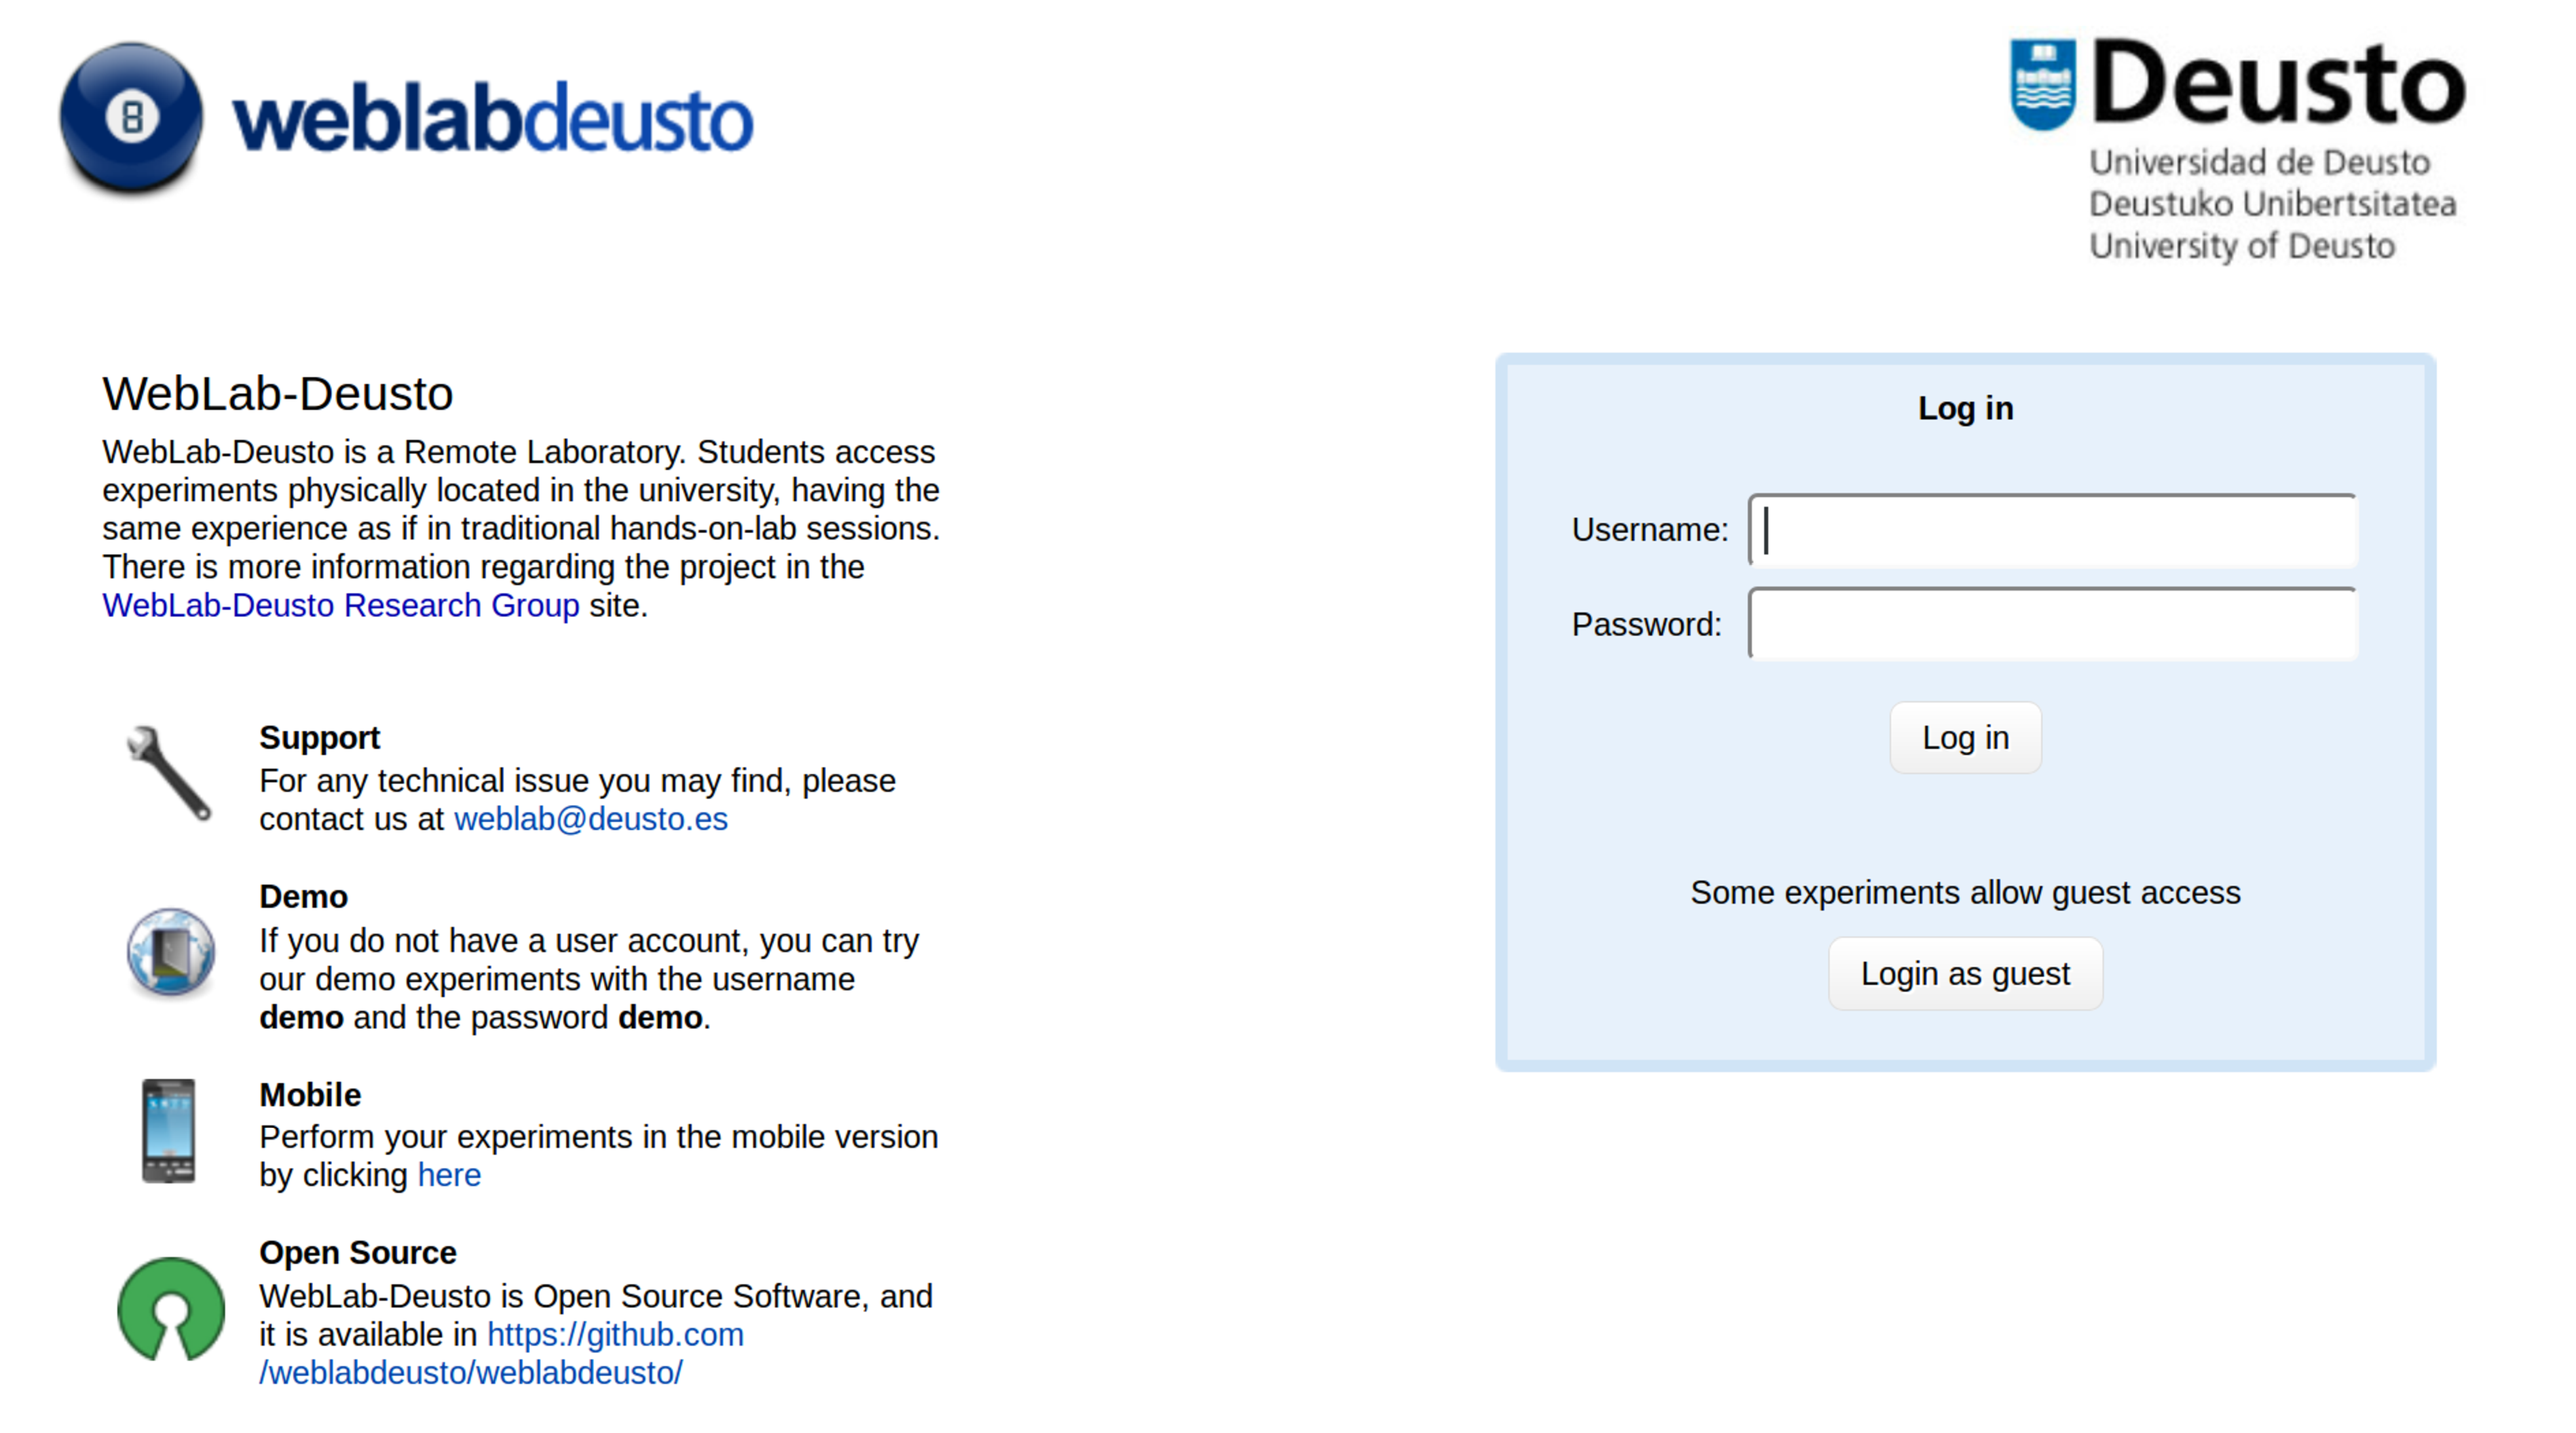
\includegraphics[width=0.75\textwidth]{fig/manuals/weblab}
	\caption{WebLab Deusto's landing page.}
	\label{fig:man:weblab}
\end{figure}

Once logged in, you will see ``romie'' experiment under the ``Robot experiments'' category
(figure~\ref{fig:man:romie_weblab}). You could see more experiments if you have the permission to
use them. If you cannot find the experiment you should contact with the administrators. Click on
``romie'' or in its image and you will enter the reservation page
(figure~\ref{fig:man:romie_reserve}). There, you can reserve the experiment clicking the ``Reserve''
button.

\begin{figure}[!htbp]
	\centering
	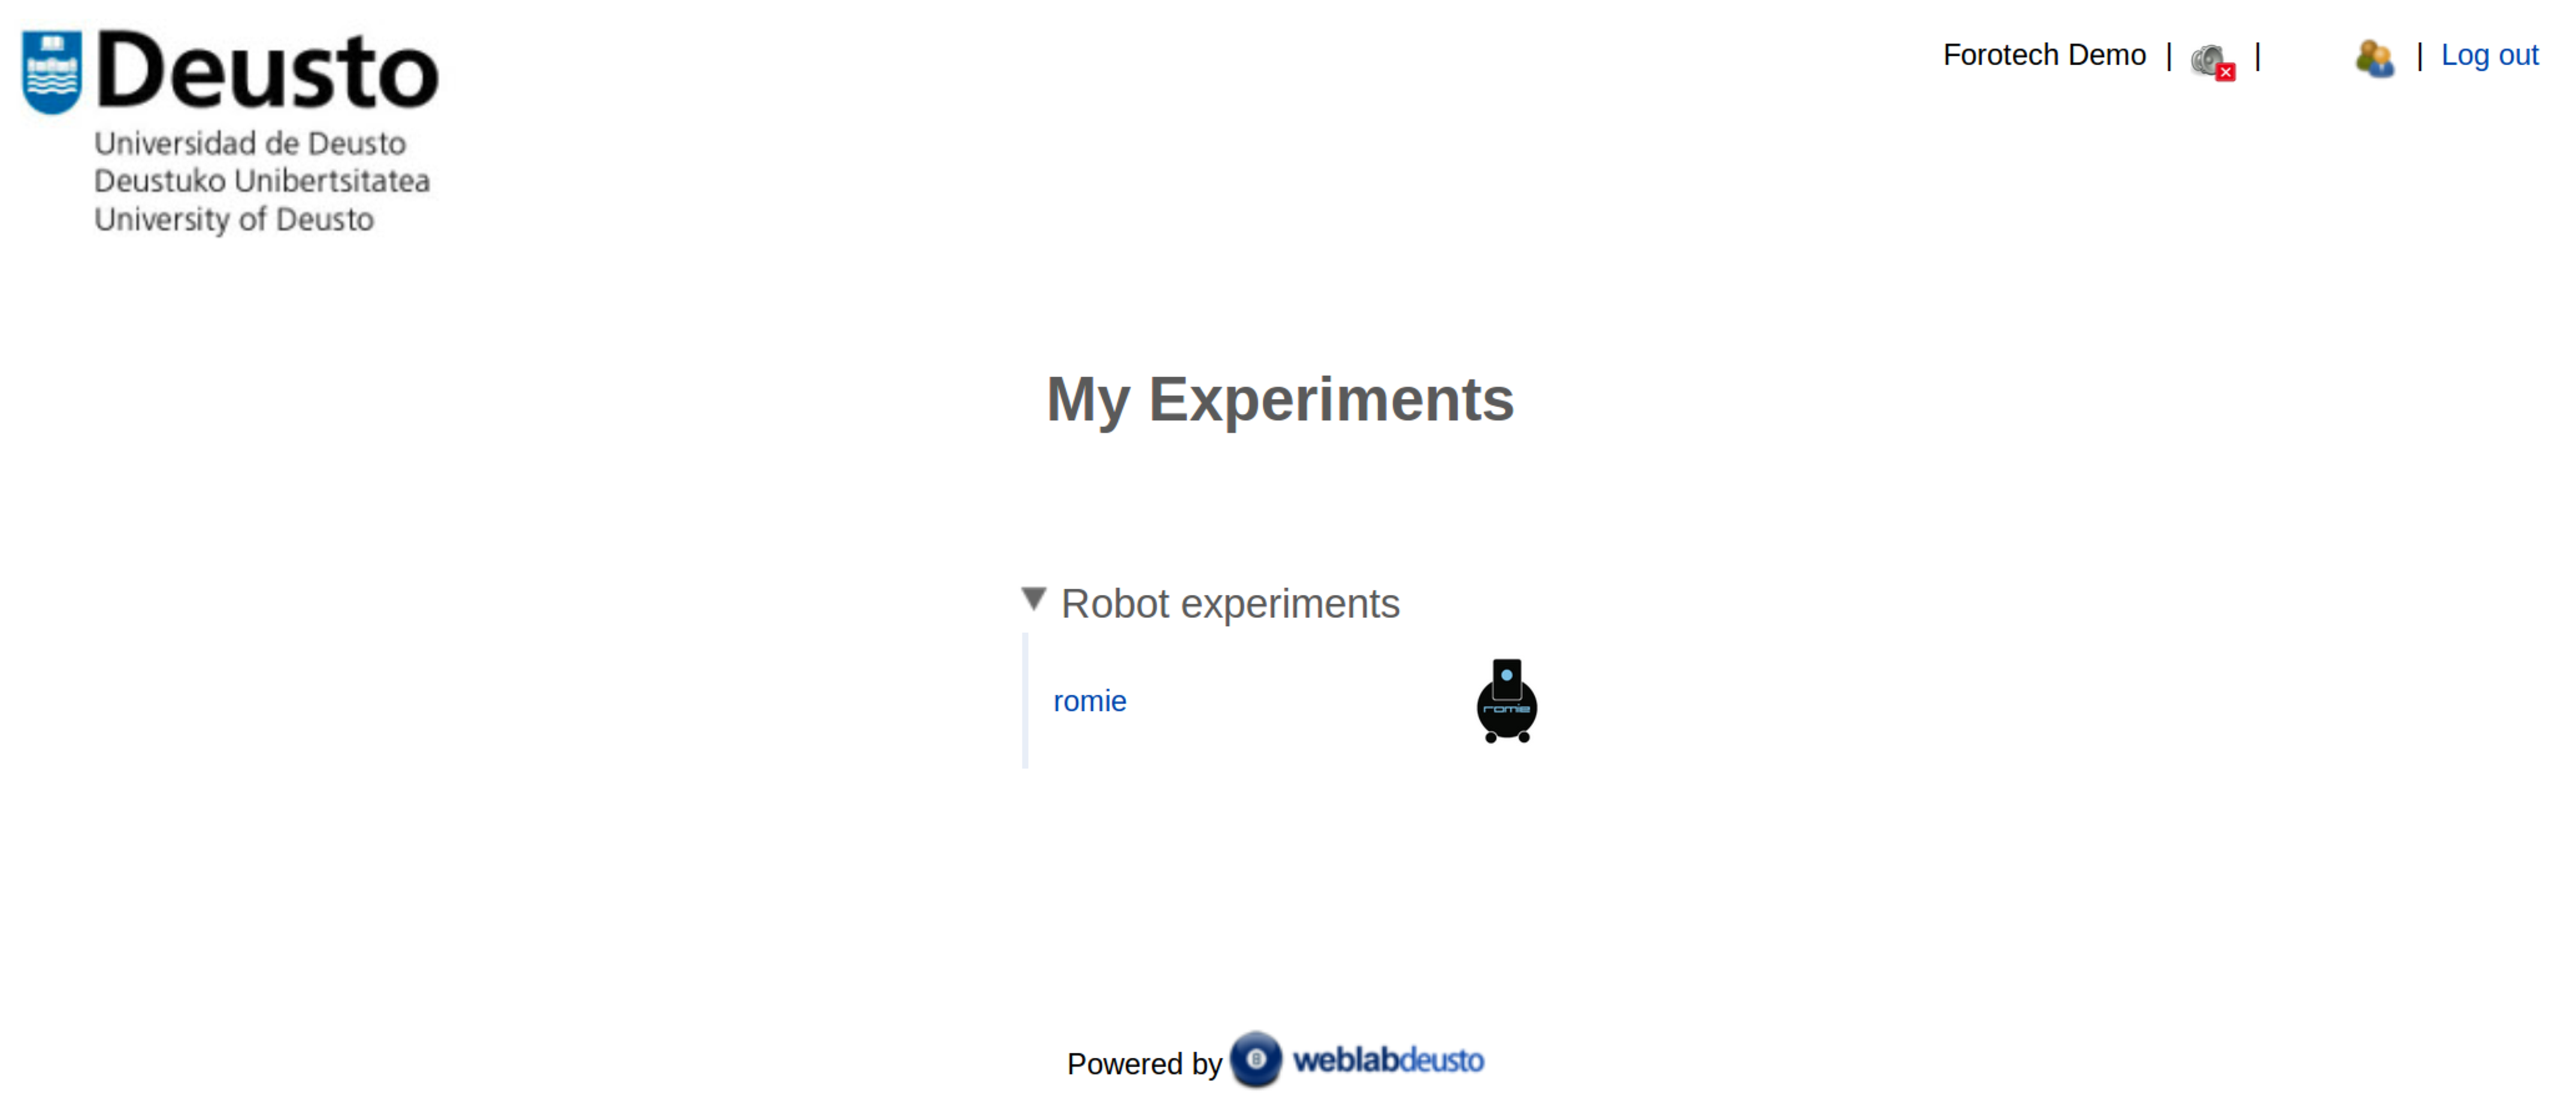
\includegraphics[width=0.85\textwidth]{fig/manuals/trivia/romie-weblab}
	\caption{Romie under ``Robot experiments'' in WebLab Deusto.}
	\label{fig:man:romie_weblab}
\end{figure}

\begin{figure}[!htbp]
	\centering
	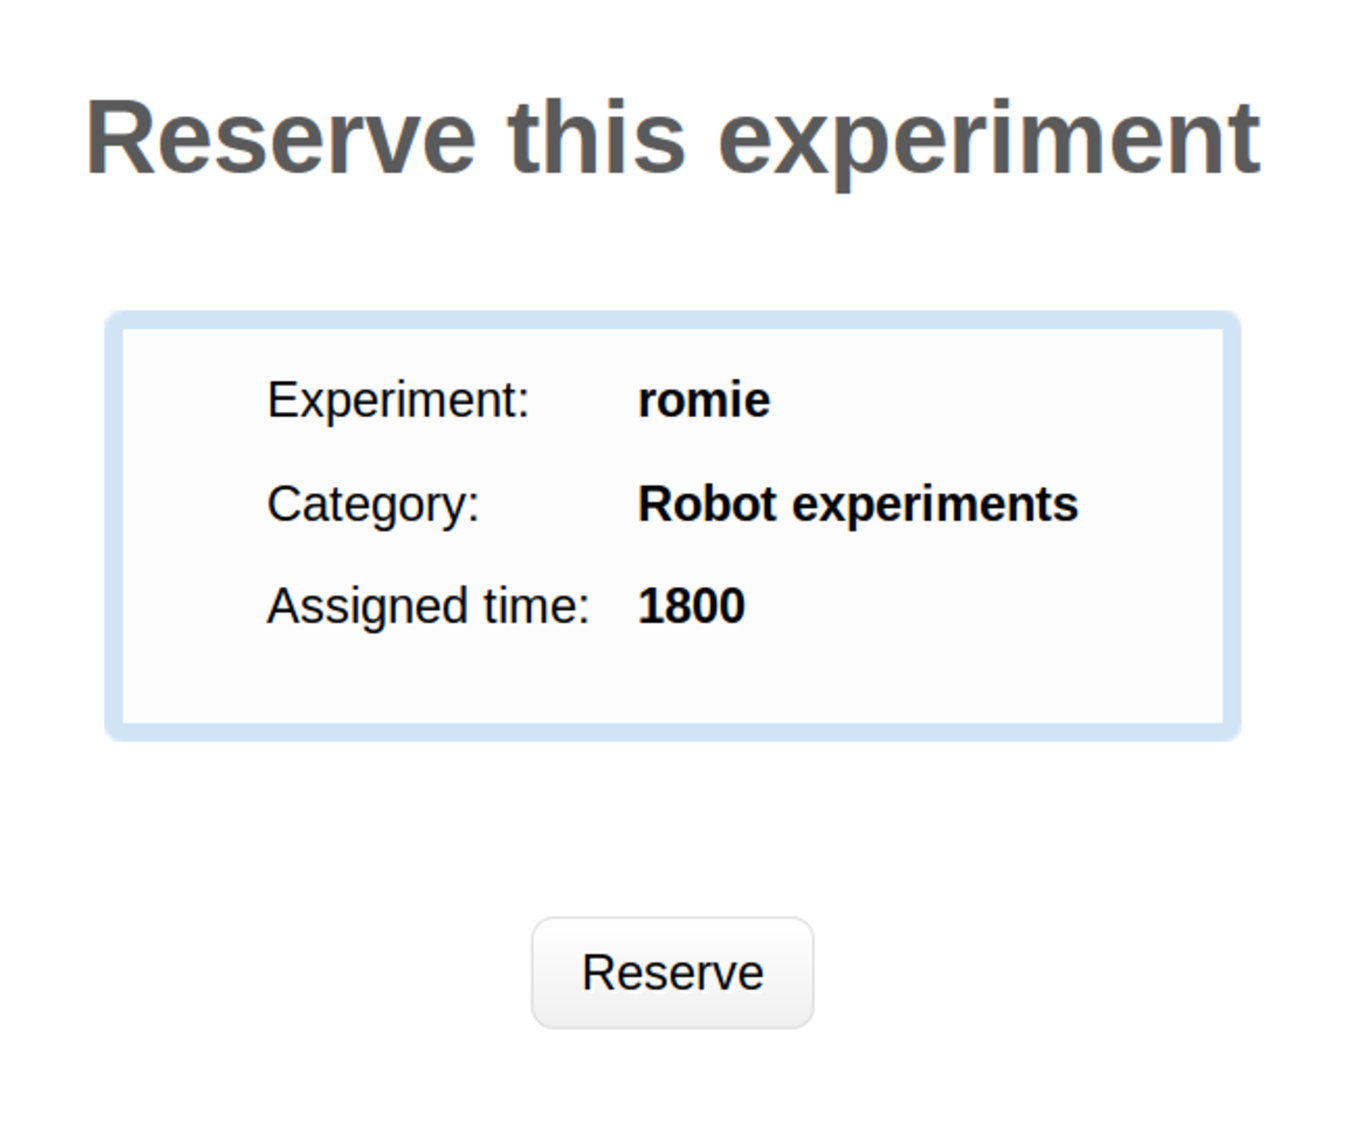
\includegraphics[width=0.5\textwidth]{fig/manuals/trivia/romie-reserve}
	\caption{Romie reservation screen.}
	\label{fig:man:romie_reserve}
\end{figure}

Once reserved, on the first use, you will see the registration form
(figure~\ref{fig:man:romie_register}). You will have to fill it in order to play the game. There is
also a version without the registration screen if you only want to test the robot, ask the
administrators for permission to use it. After filling the registration form  with your own data,
you can click the register button. \emph{Note: the experiment is prepared to work with students of
less than 18 years old, so any age above that or below 5 years old is considered an input error,
that will be notified in the interface}.

\begin{figure}[!htbp]
	\centering
	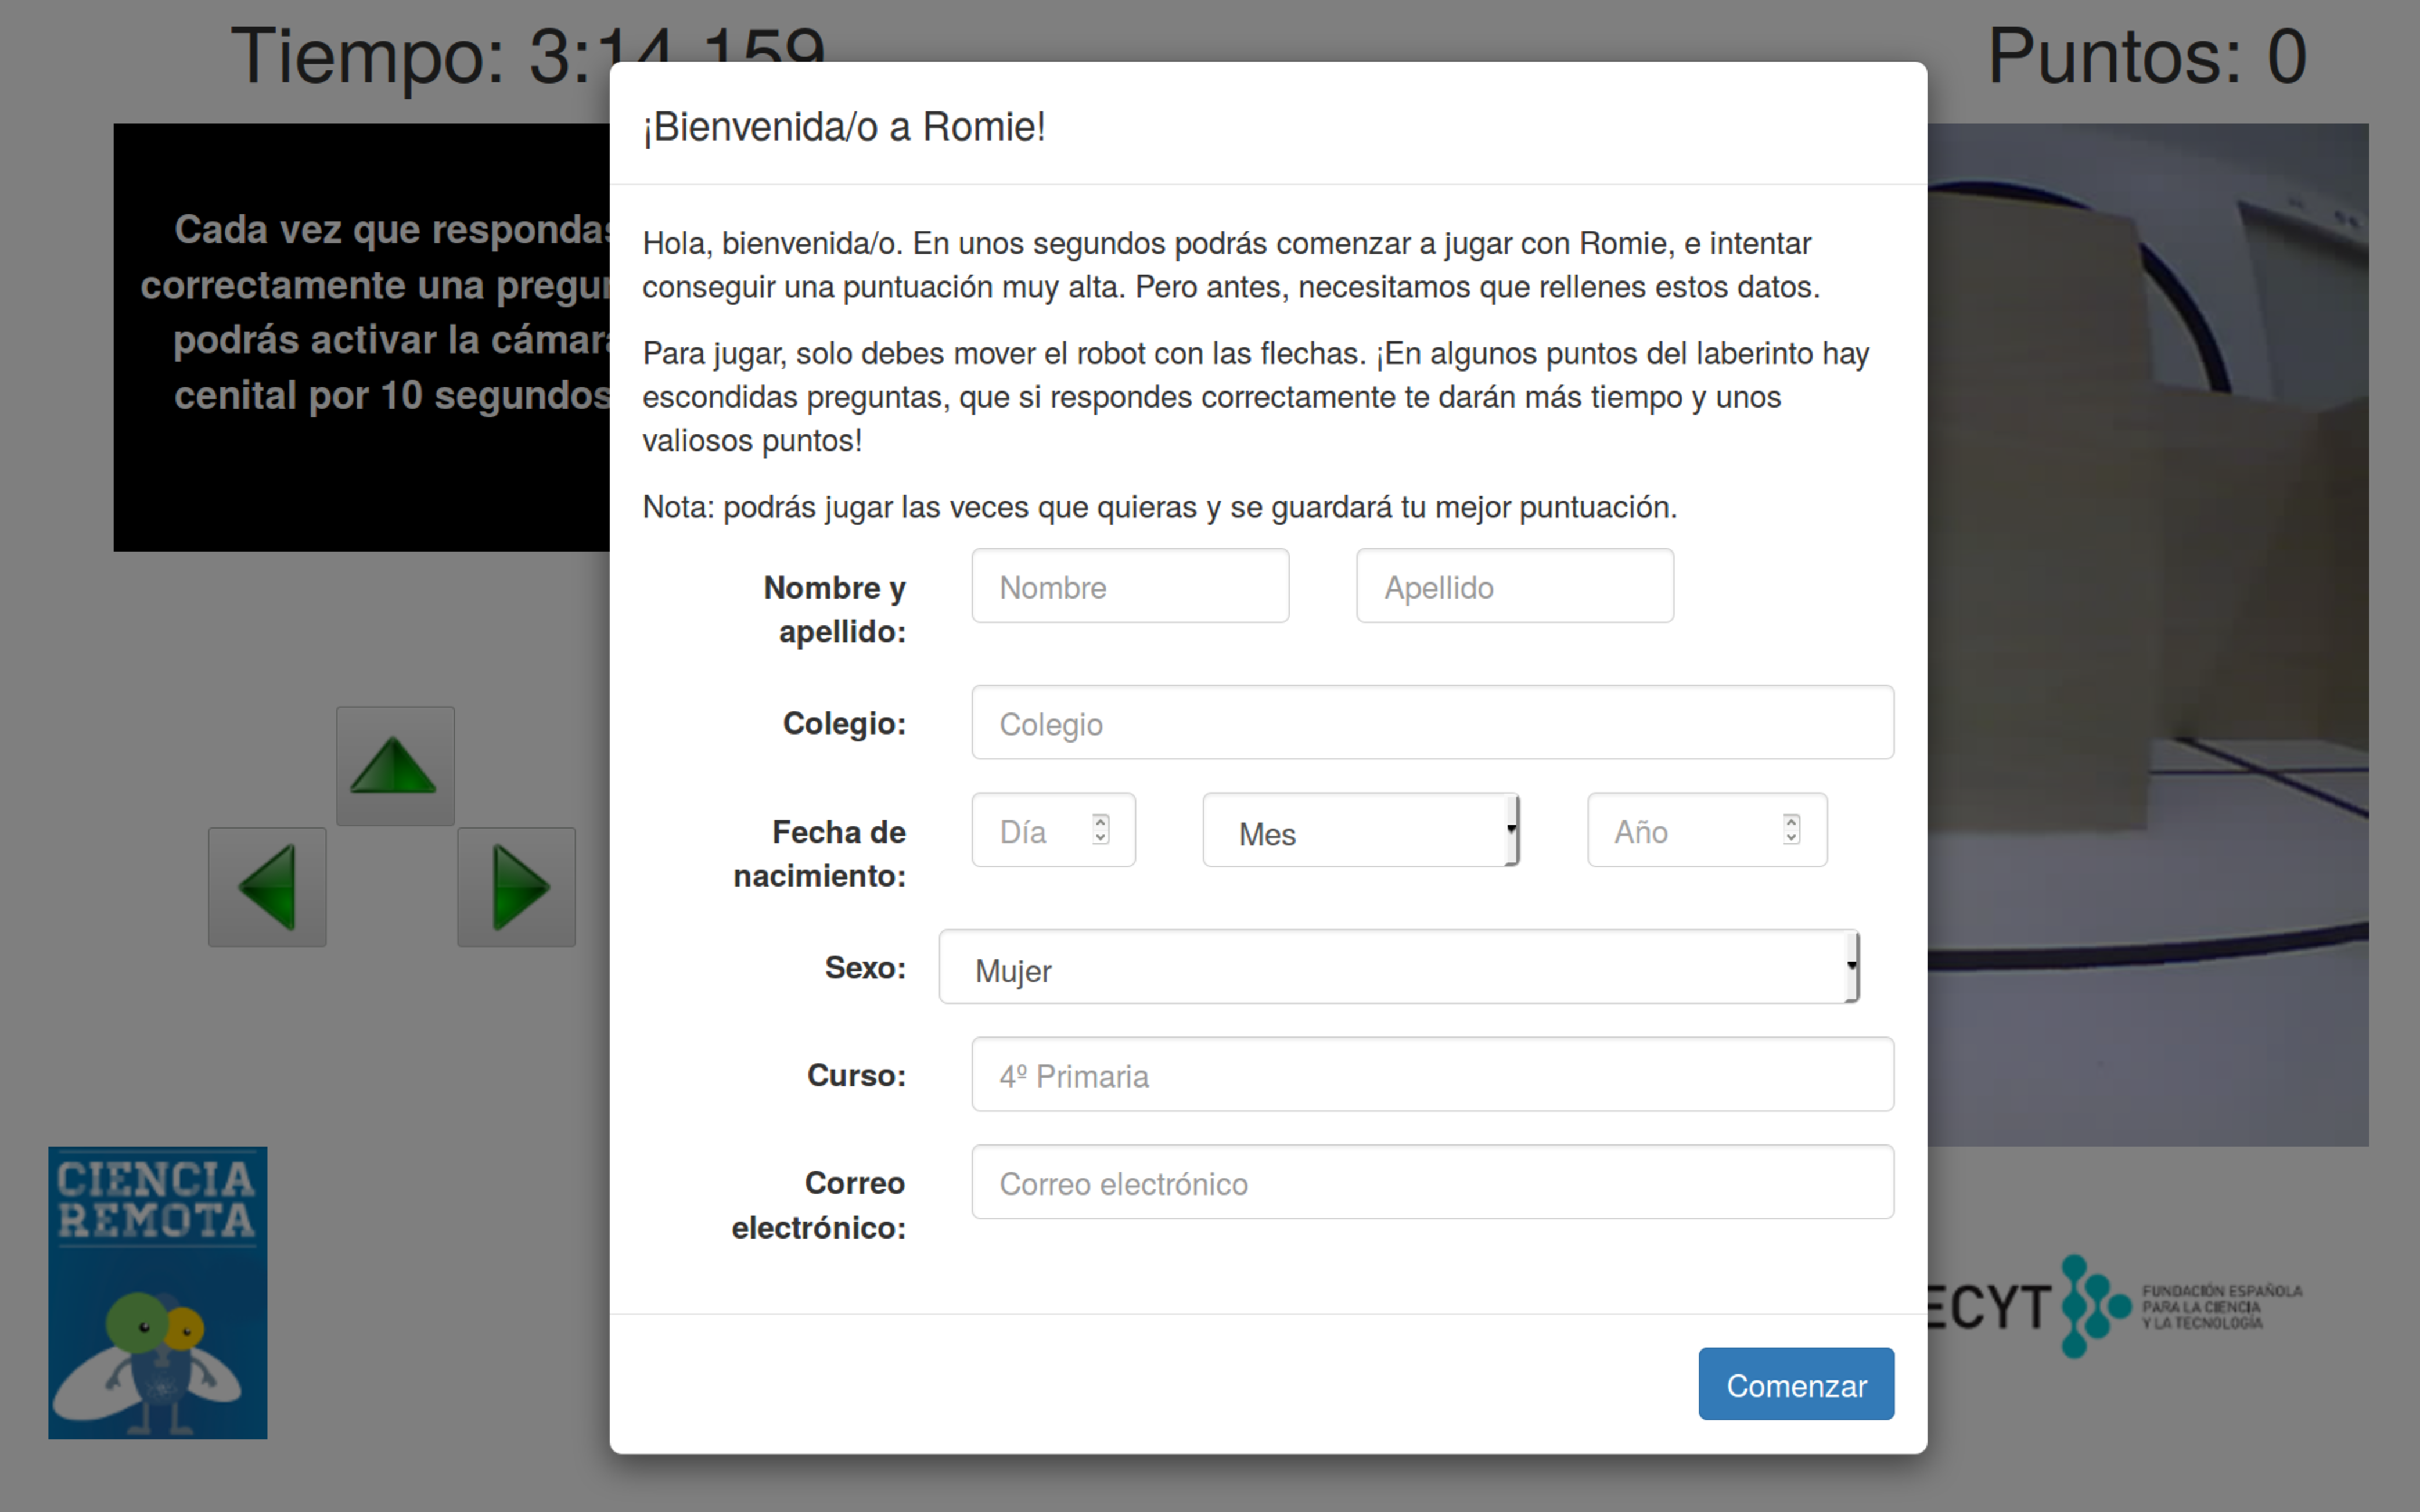
\includegraphics[width=0.85\textwidth]{fig/manuals/trivia/romie-register}
	\caption{Romie's registration form.}
	\label{fig:man:romie_register}
\end{figure}

After the registration, you will be able to play with Romie. The game is pretty easy to use: you
will have three arrows in the left control pad (figure~\ref{fig:man:romie_start}), where you will be
able to click and command the robot to move forward or to turn left or right. Moreover, you will
have the on-board camera to see what the robot does. If you press forward against a wall do not
worry, the robot will not collide.

\begin{figure}[!htbp]
	\centering
	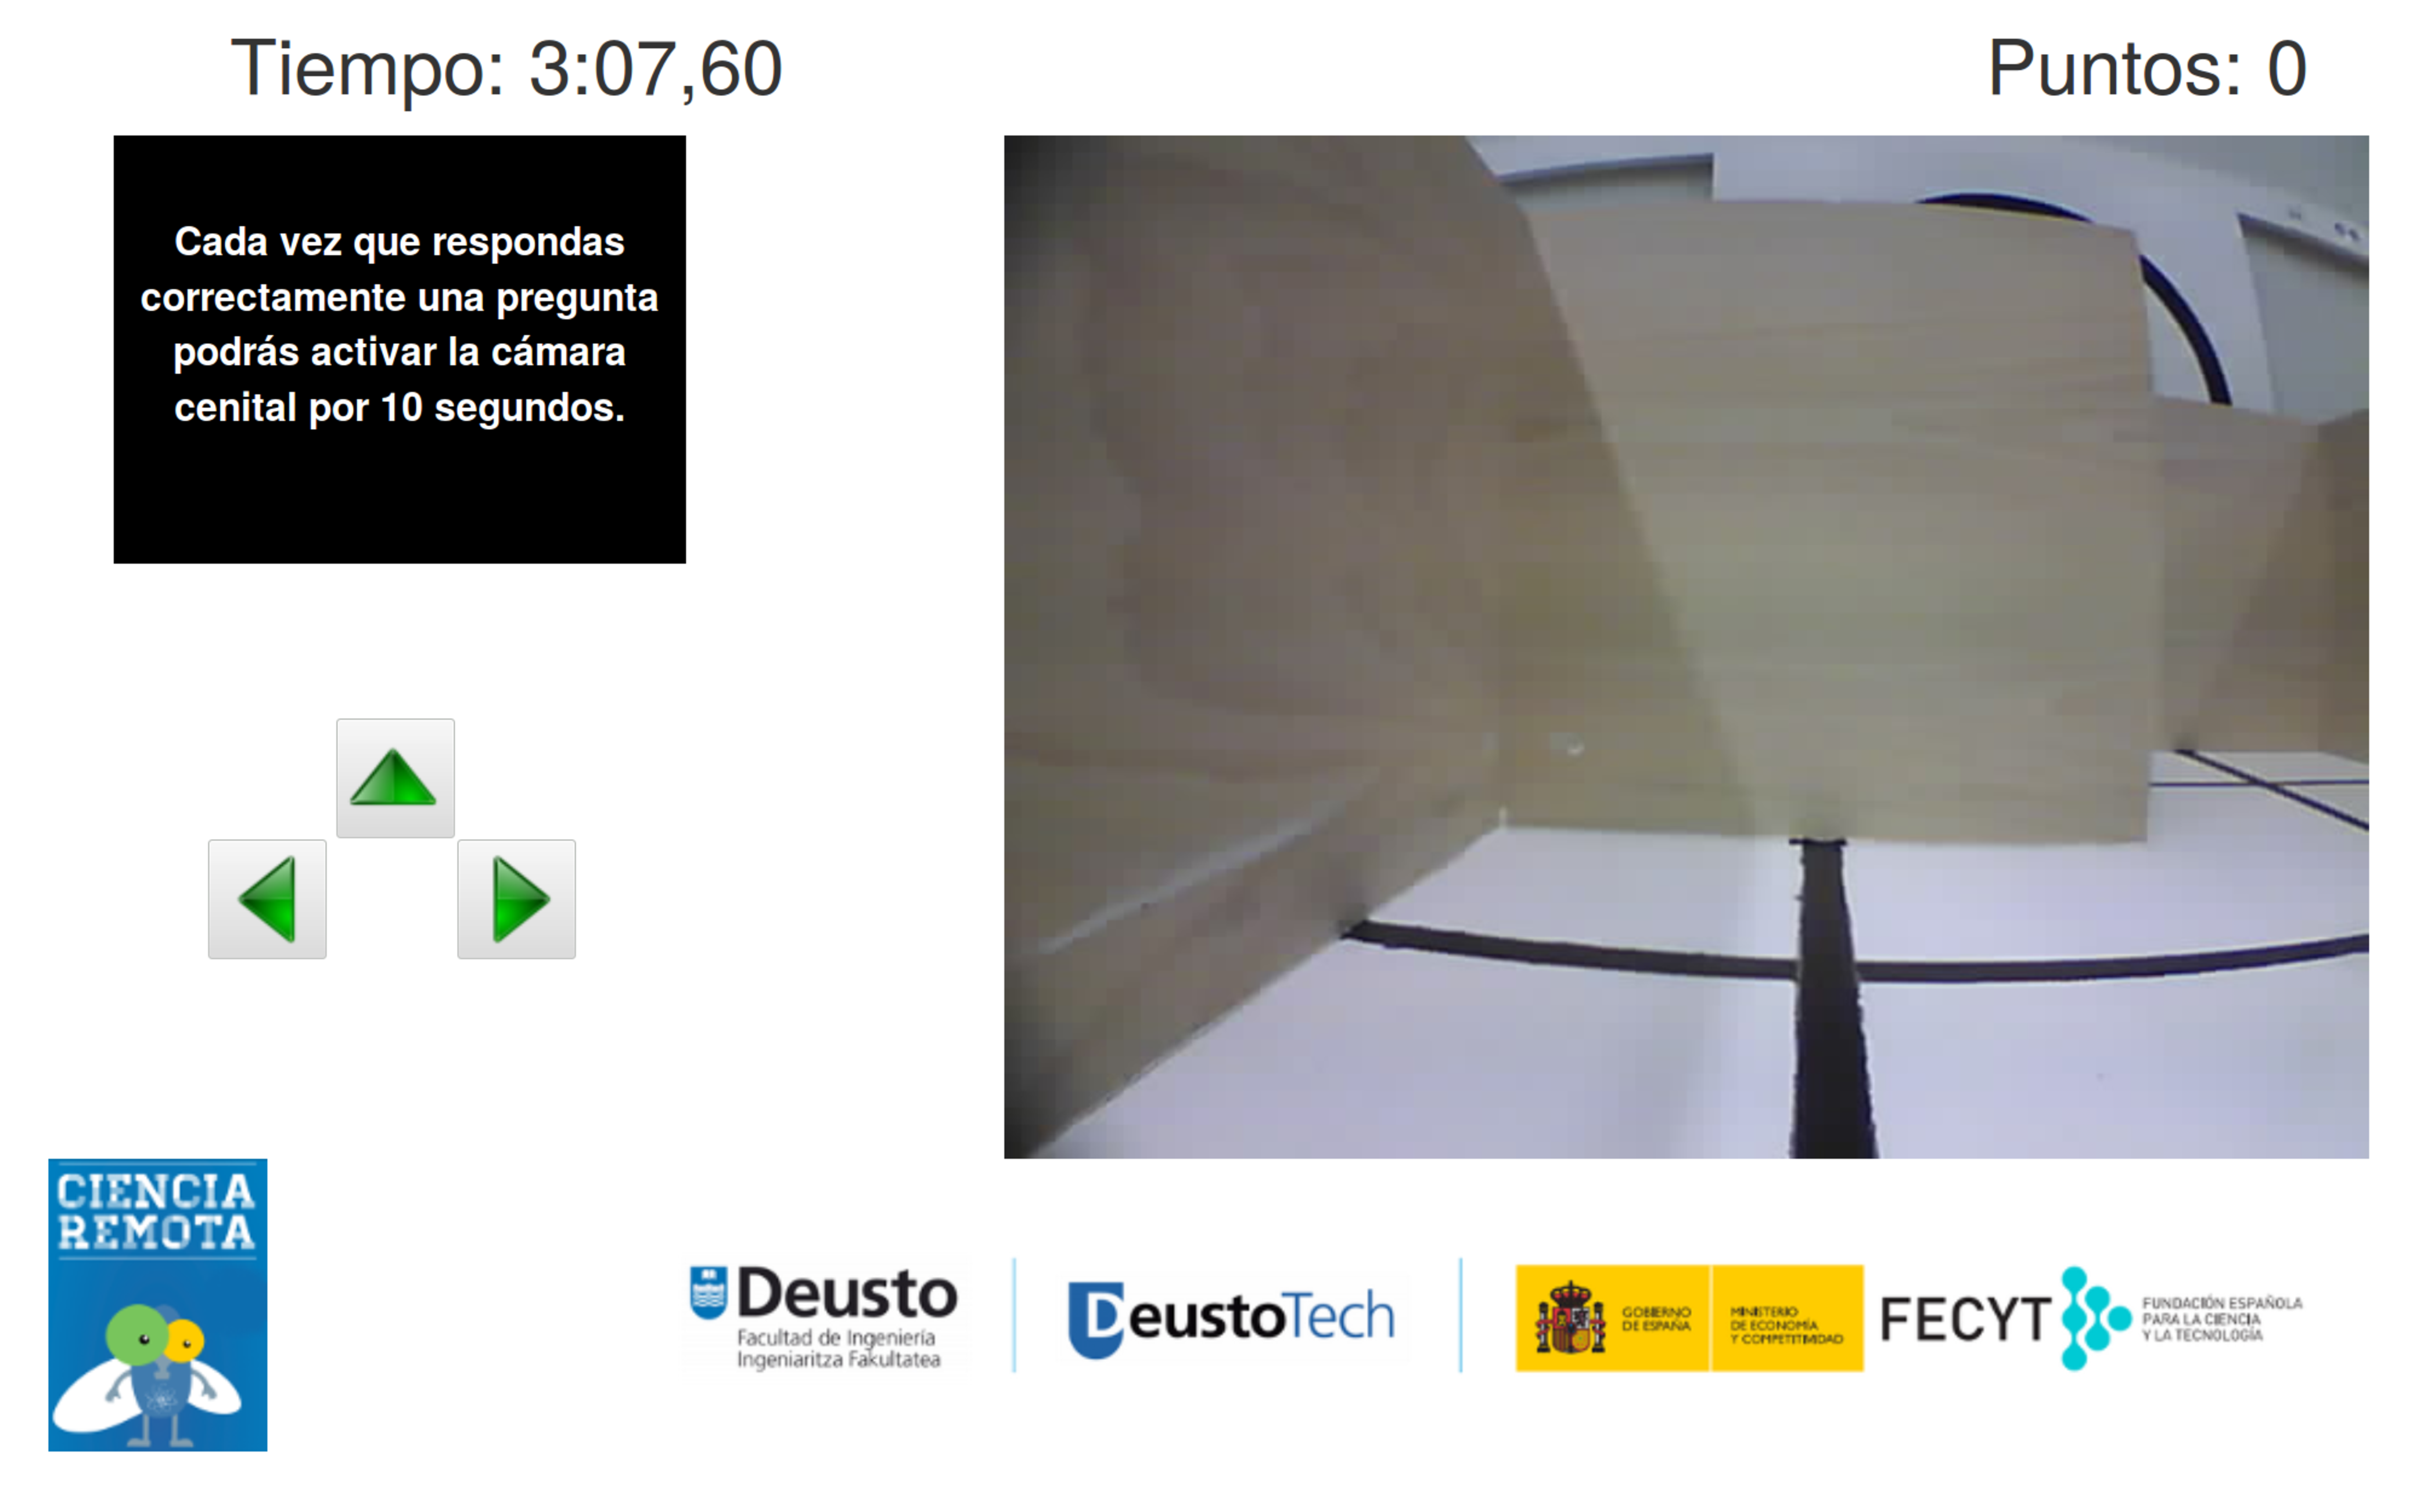
\includegraphics[width=0.85\textwidth]{fig/manuals/trivia/romie-start}
	\caption{Playing with Romie.}
	\label{fig:man:romie_start}
\end{figure}

If you fall in top of a card, you will be asked a question (figure~\ref{fig:man:romie_question}). If
you answer correctly, you will be given points and more time to continue playing. Furthermore, you
will have the opportunity to manually activate the ceiling camera to see all the labyrinth and
decide where to go (figure~\ref{fig:man:romie_ceiling}).

\begin{figure}[!htbp]
	\centering
	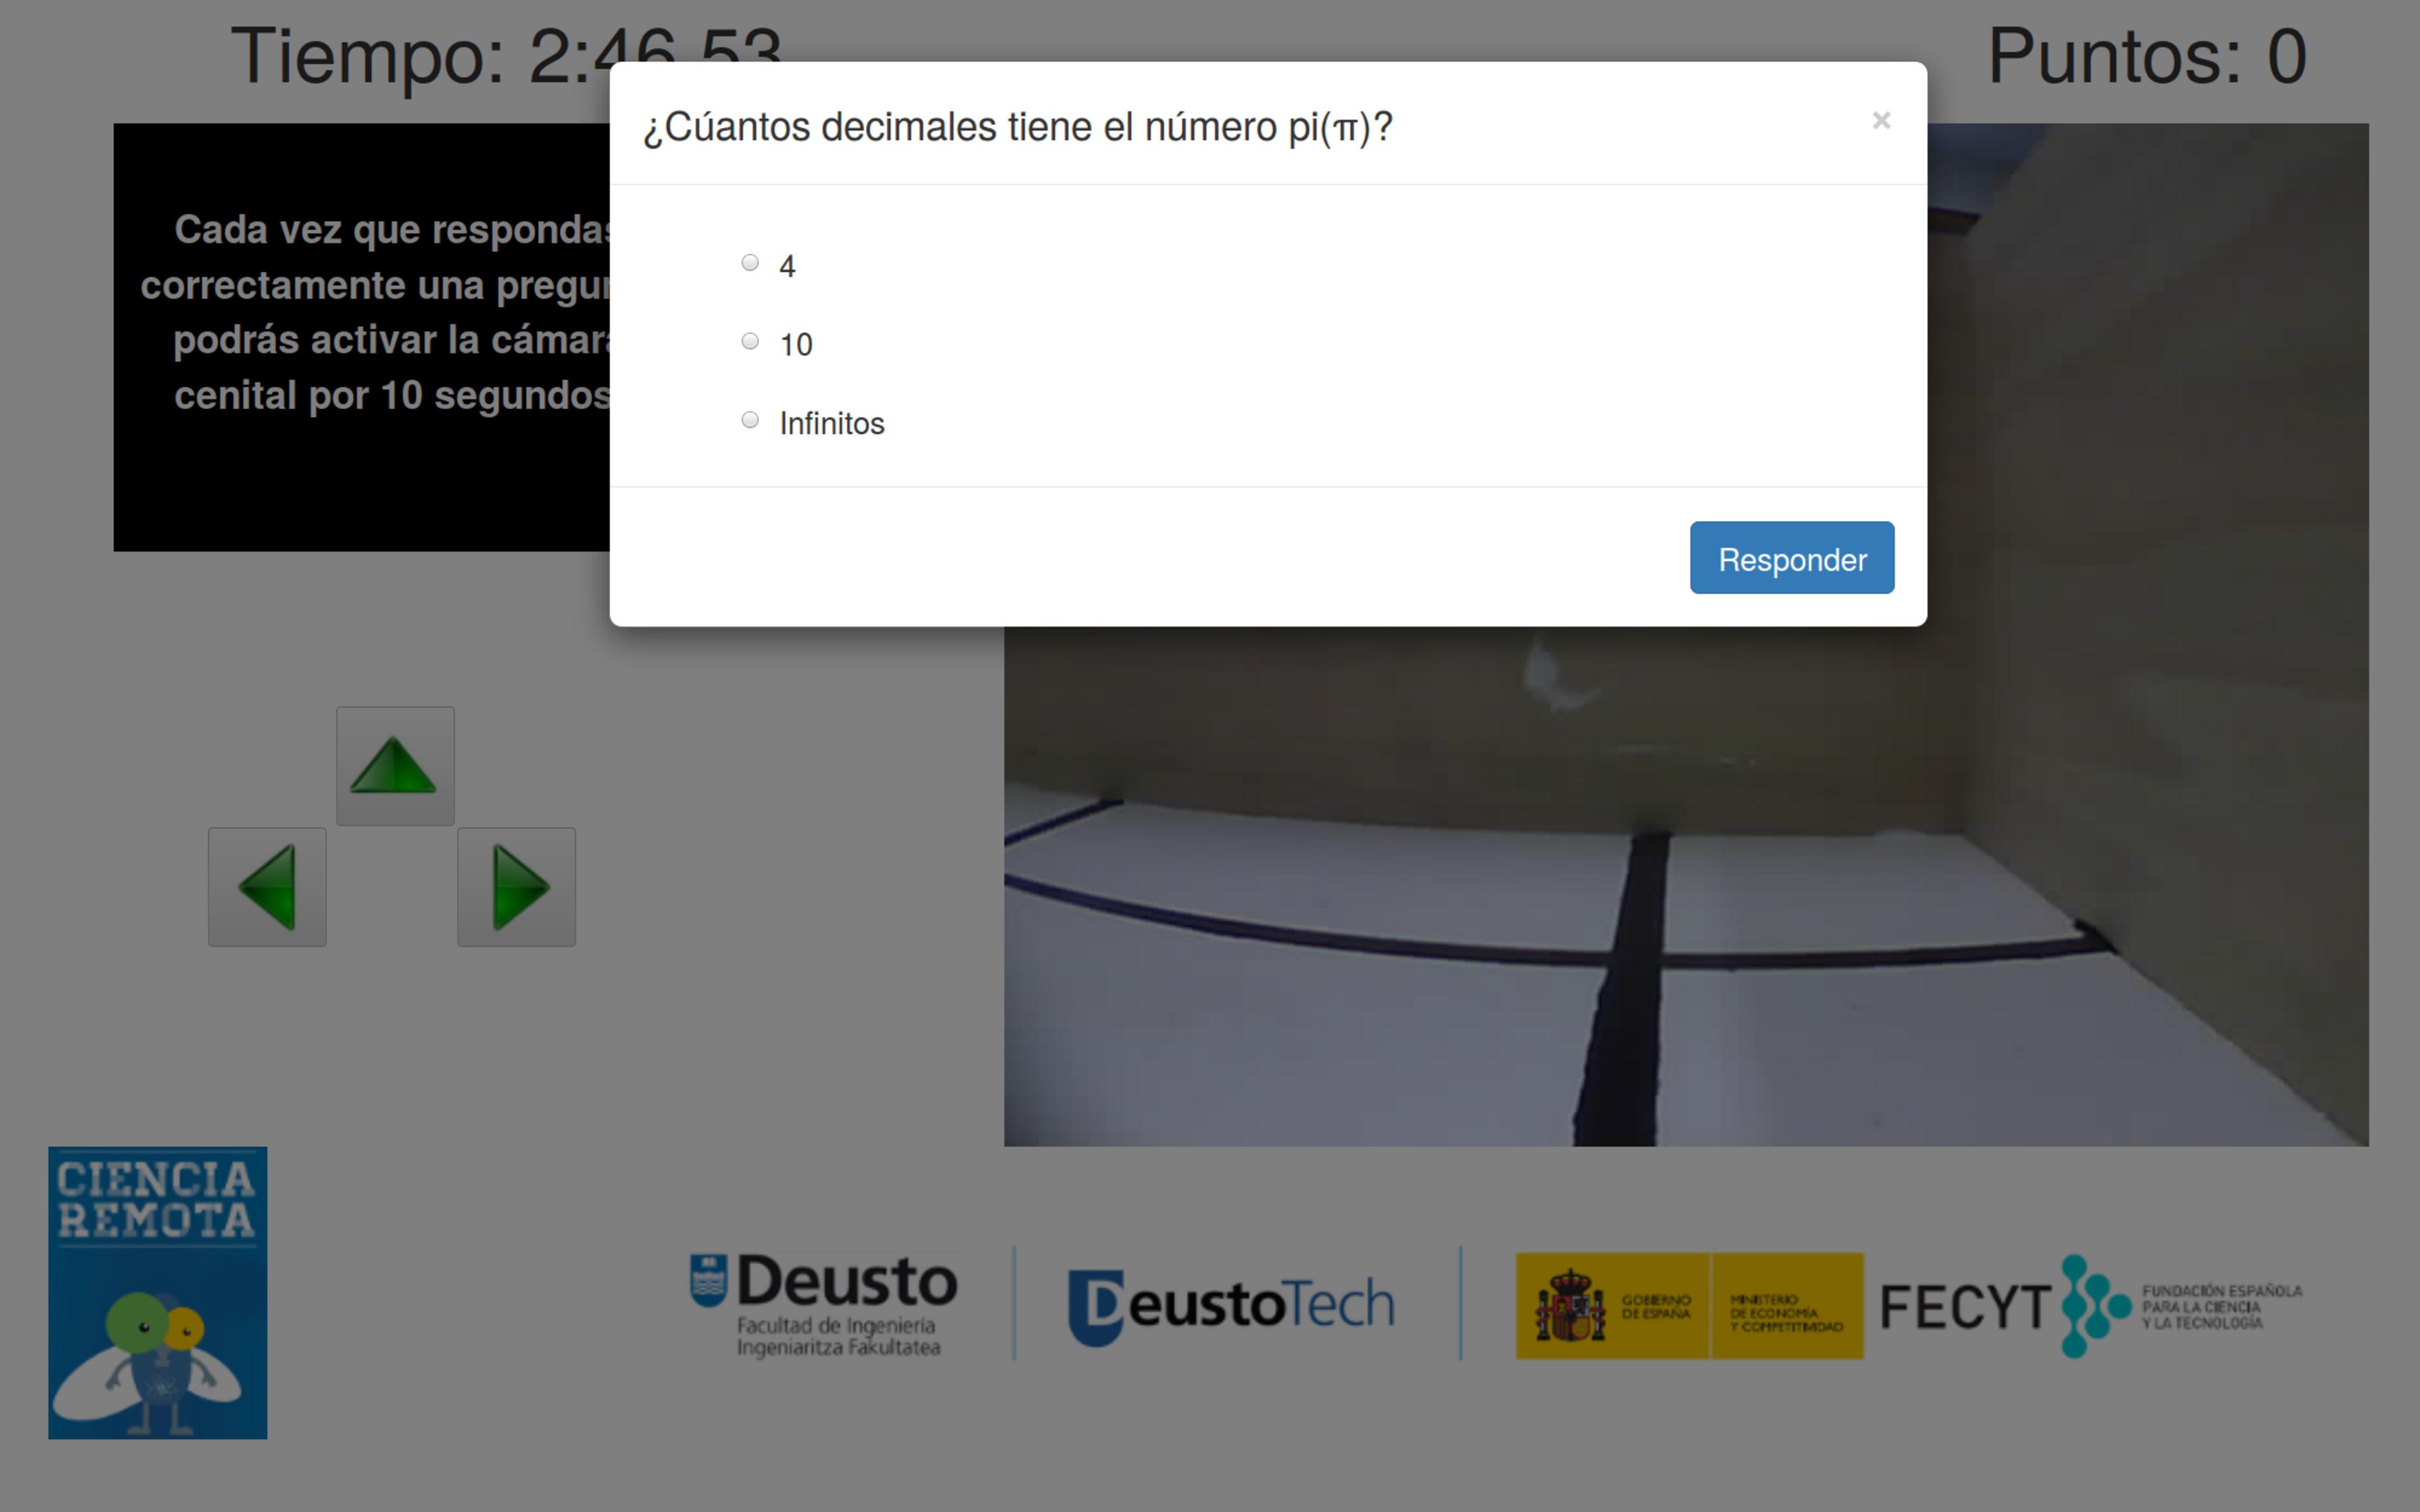
\includegraphics[width=0.85\textwidth]{fig/manuals/trivia/romie-question}
	\caption{Romie asks you questions when you drive onto a card.}
	\label{fig:man:romie_question}
\end{figure}

\begin{figure}[!htbp]
	\centering
	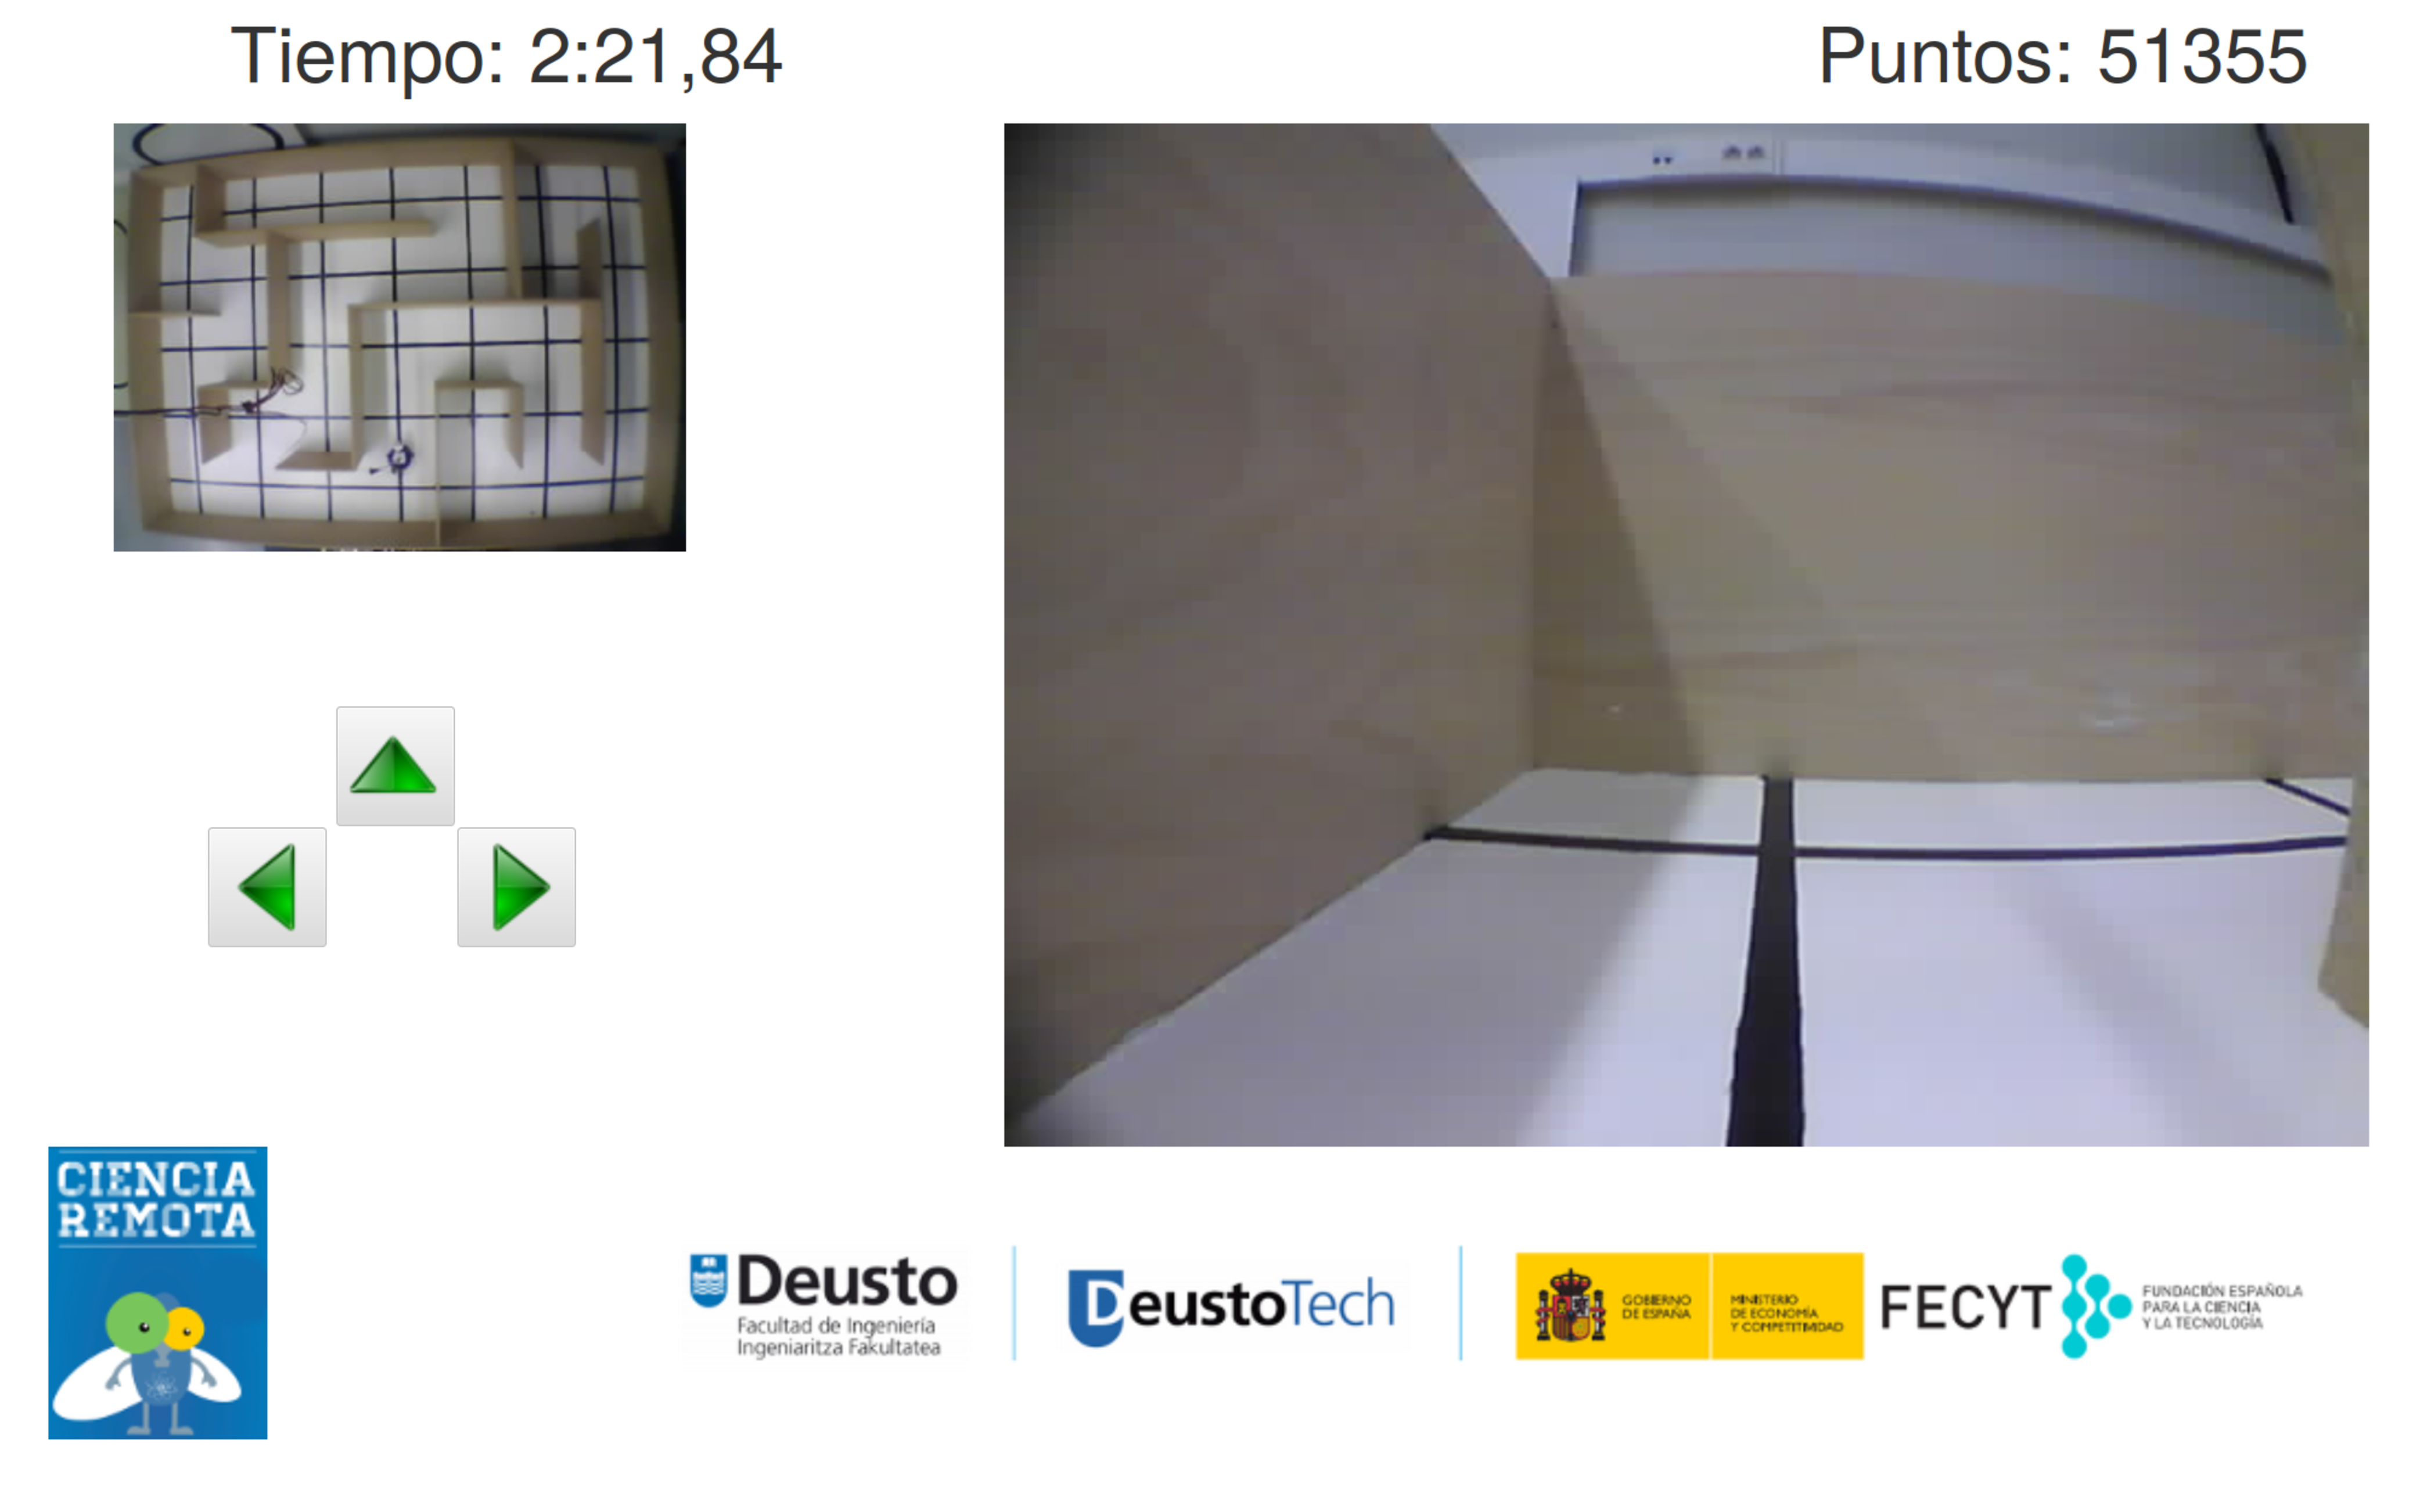
\includegraphics[width=0.85\textwidth]{fig/manuals/trivia/romie-ceiling}
	\caption{You can activate the ceiling camera when you answer a question correctly.}
	\label{fig:man:romie_ceiling}
\end{figure}

Finally, when the time finishes, you will see a ranking with the 10 best scores of the game (less if
there has not been enough users) with your user selected in green if you are in the top ten, as you
can see in figure~\ref{fig:man:romie_ranking}.

\begin{figure}[!htbp]
	\centering
	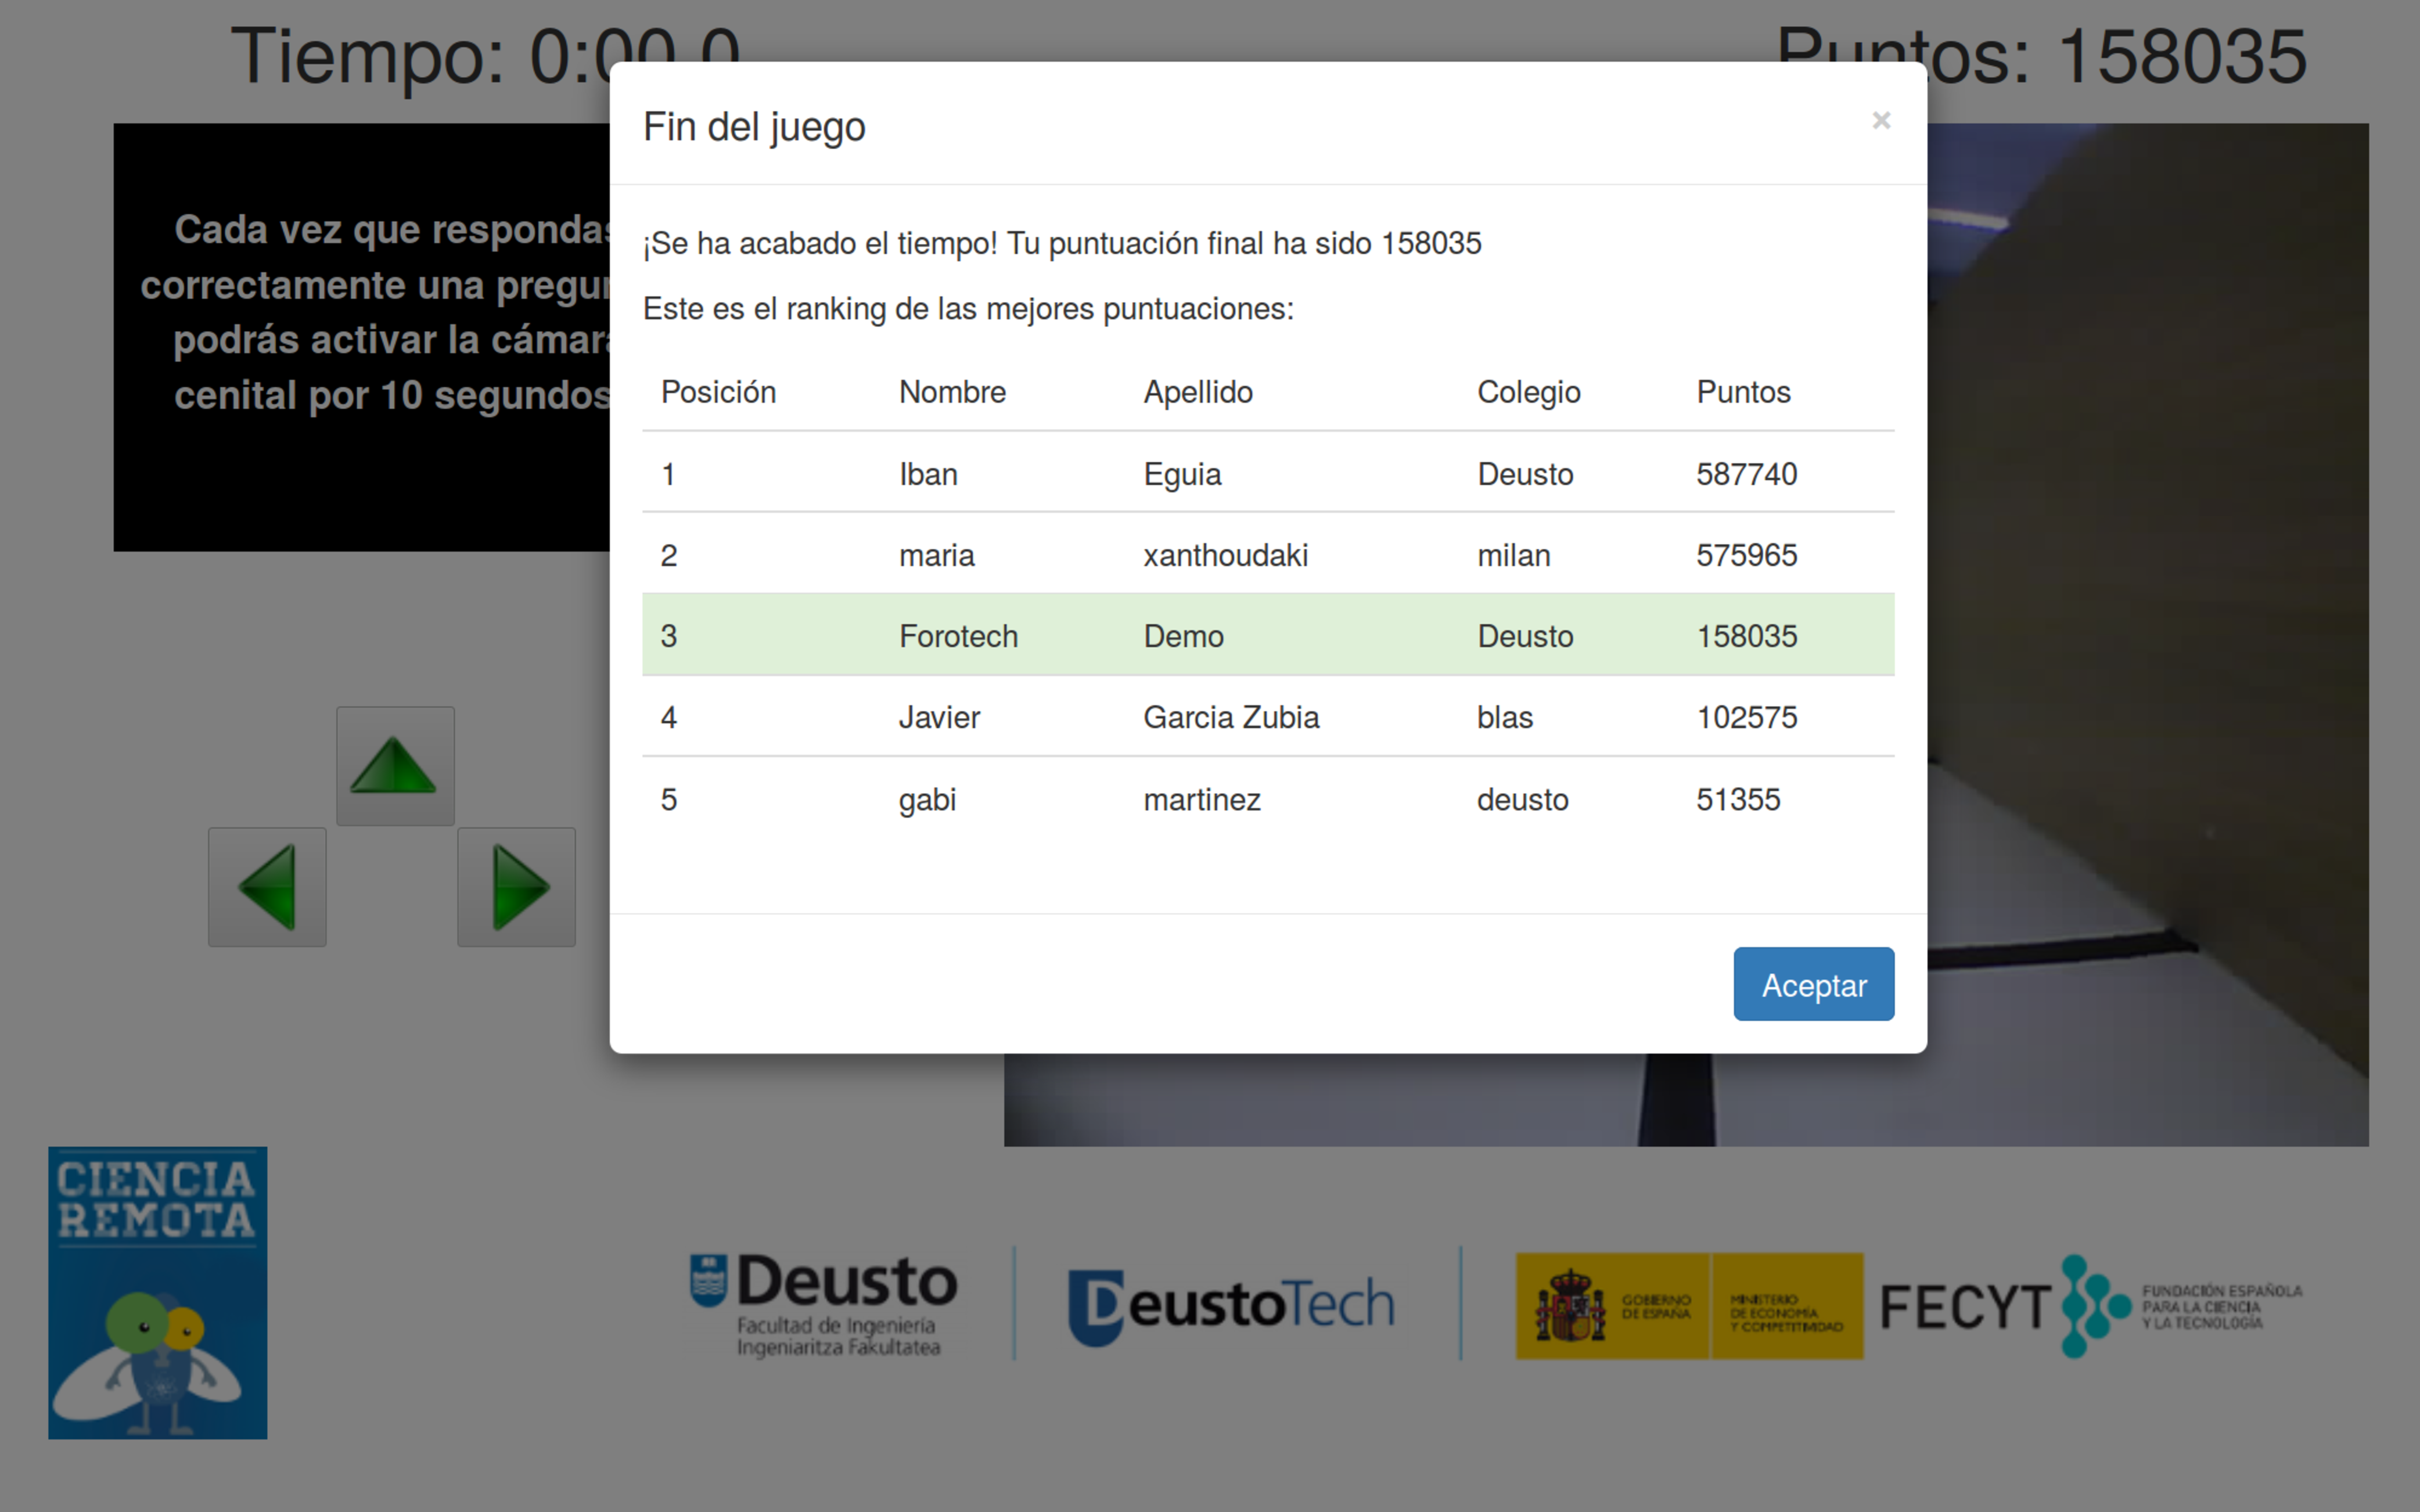
\includegraphics[width=0.85\textwidth]{fig/manuals/trivia/romie-ranking}
	\caption{The final ranking where you can see the best scores.}
	\label{fig:man:romie_ranking}
\end{figure}

\subsection{Issue Management}

During the development we have faced some issues that we have had to deal with. One of the first
issues we had was that the robot was not reading the lines properly, mainly the ones in the
intersections. That was caused because the contrast between the line and the background was
insufficient. We solved it by painting all the labyrinth in white and adding the lines in black
painting them. That way we did not need to use tape and the robot started to work properly.

Other issue we found was that the robot did not read the \acrshort{rfid} tags every time it went on
top of them. The problem was that the \acrshort{rfid} reader we were using, the ID-12 seemed to have
some working issues, since the reader was located about 10-15~mm from the floor. We decided to
change it by a ID-20 reader, that has a 180~mm range~\cite{rfid} and worked perfectly.

Furthermore, we had the problem with electricity, that it was using batteries, and as we have seen
above, we had to change it to cables. The main issue was that the cables would get entangled with
the walls. We solved it by extending a flexible artifact in top of the robot
(figure~\ref{fig:lines}).

\begin{figure}[!htbp]
	\centering
	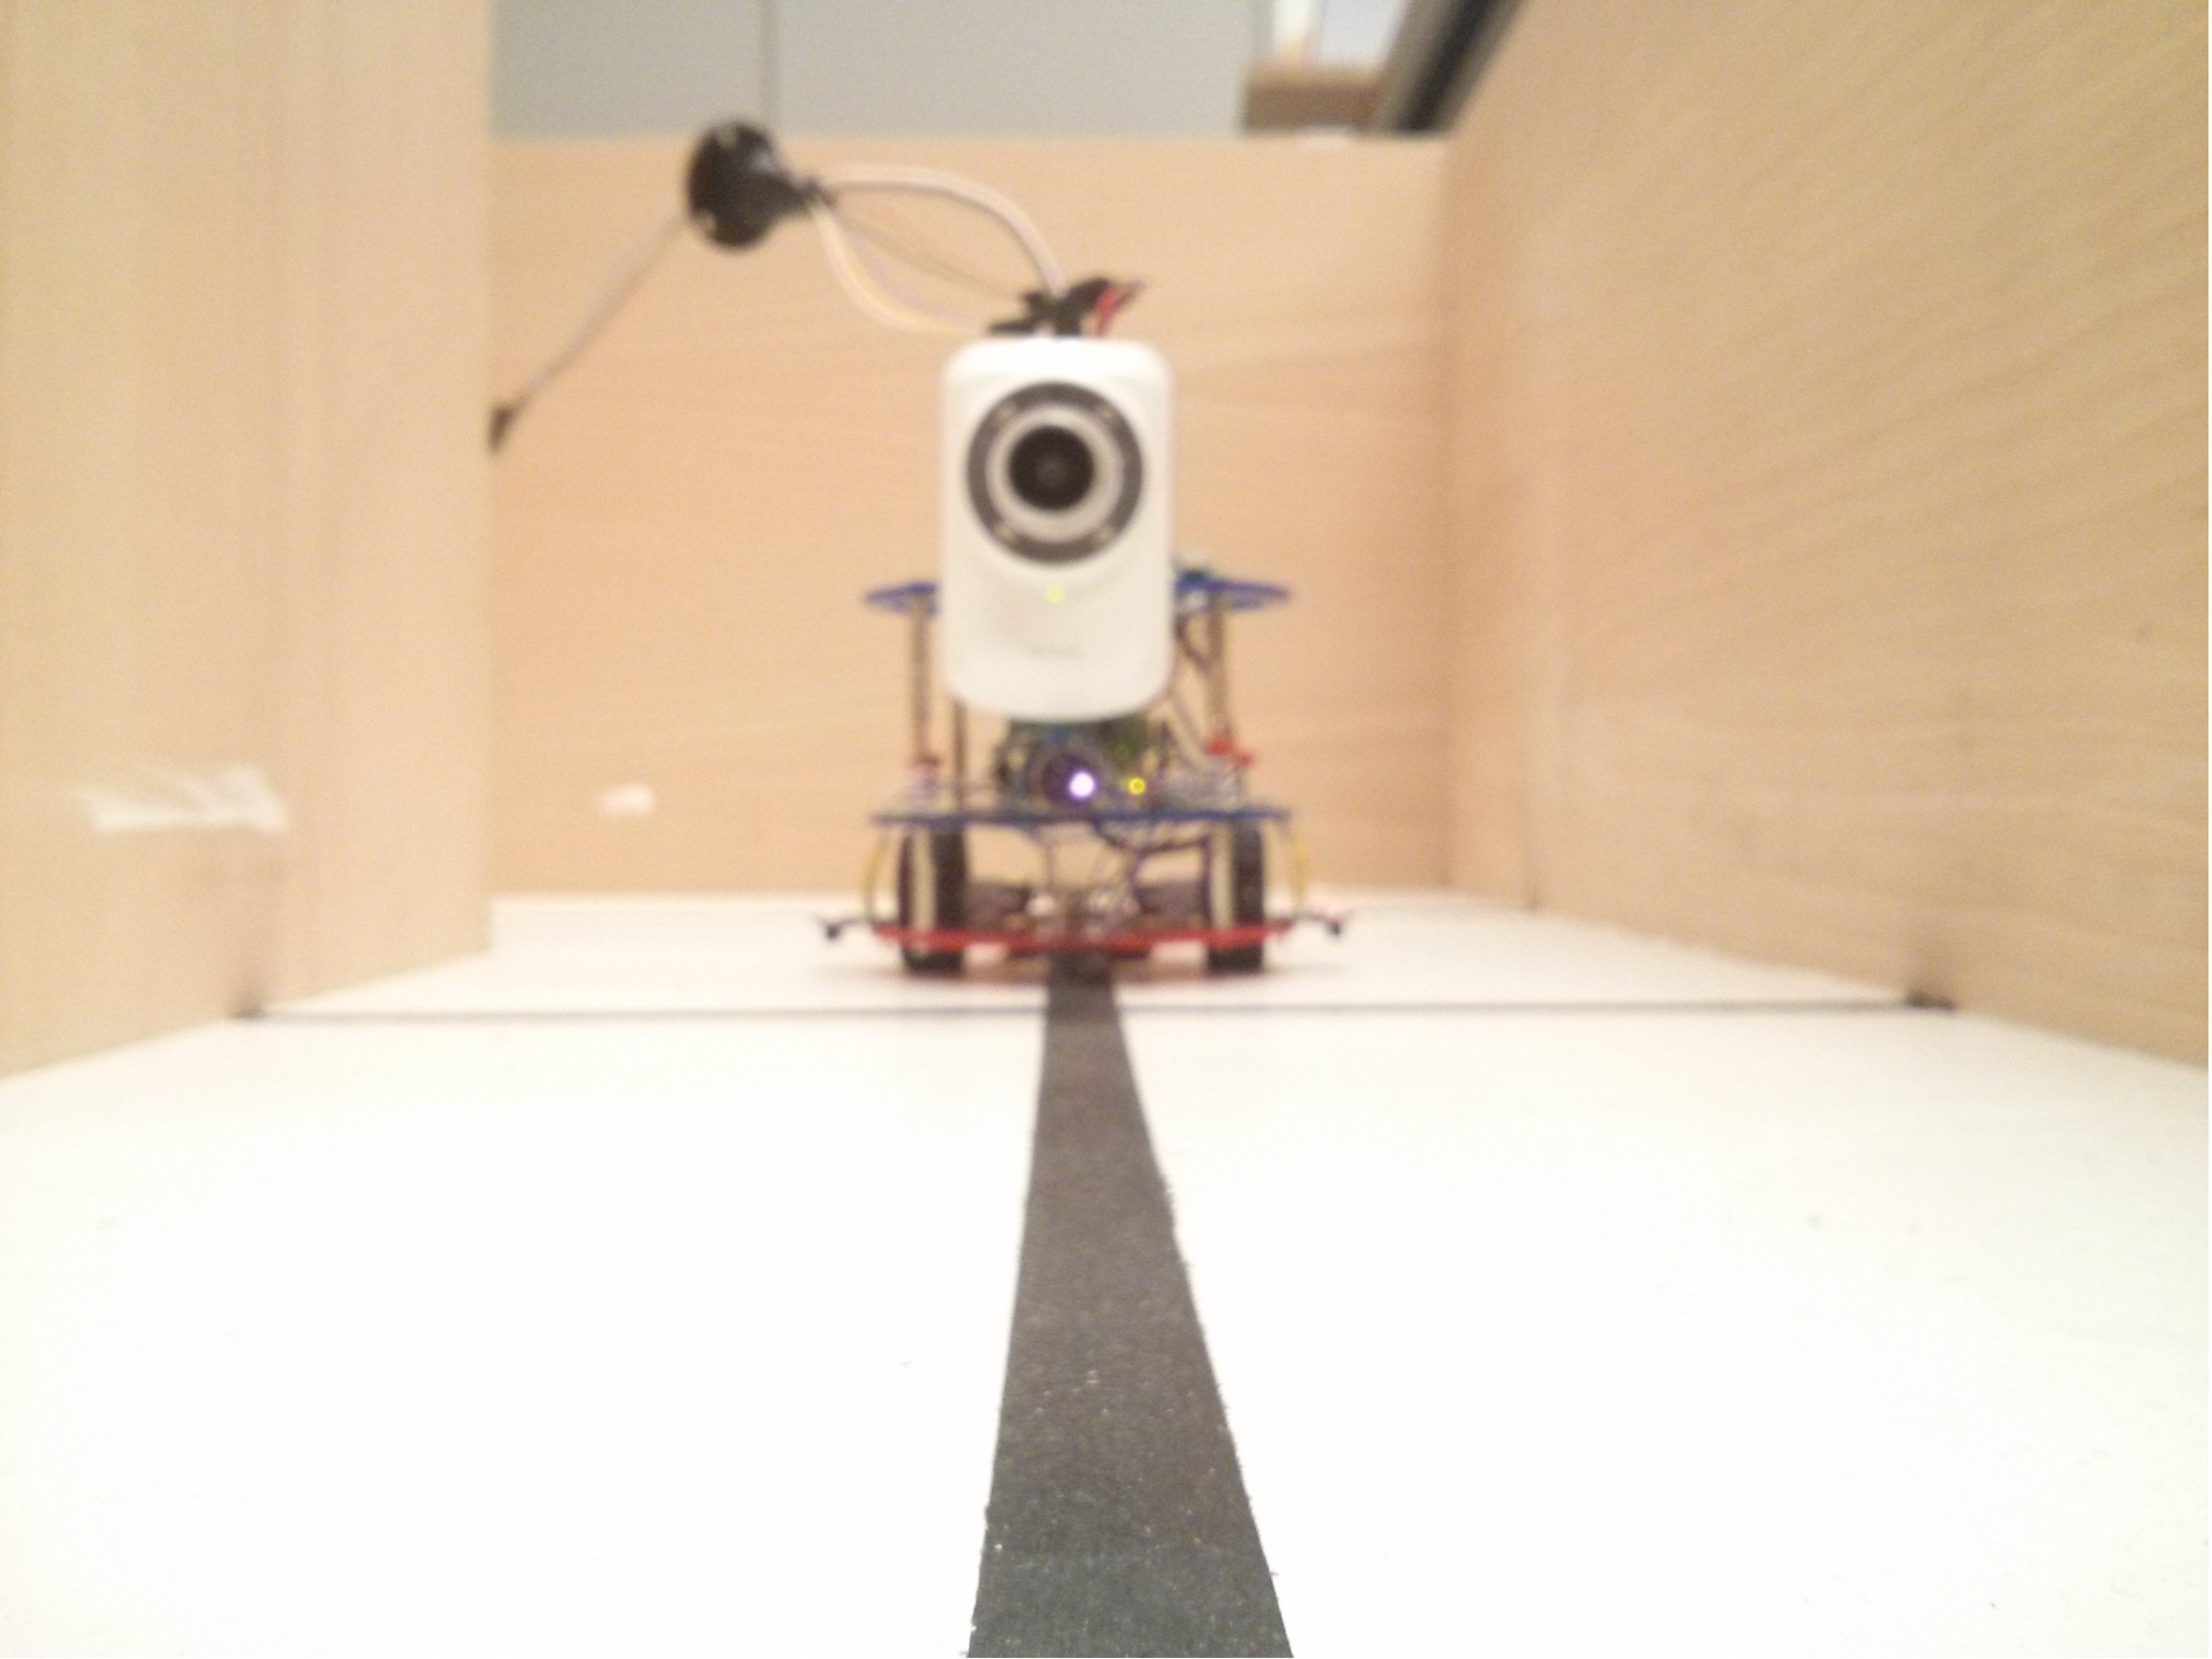
\includegraphics[height=0.35\textheight]{fig/lines}
	\caption{Romie must not get entangled with the walls.}
	\label{fig:lines}
\end{figure}

Finally, we had a problem with the wall sensor, since it would disconnect sometimes. This was a
hardware issue that we could not solve easily, since the sensor would arrive at least 1 month after
being requested. Taking that into account we decided to implement a software solution directly in
the robot so that it would go back automatically if something went wrong, as we can see in
algorithm~\ref{alg:romie_wall}.

\begin{center}
\begin{minipage}{.9\textwidth}
\singlespace
\begin{pyglist}[language=c, caption={Arduino code for returning if wall was hit.},
	label={alg:romie_wall}, listingname={Algorithm}, numbers=left]
if (millis()-lastTimeFollow >= 8000) {
	while(digitalRead(FLIline) == HIGH) Motors.turnRight(100);
	while(digitalRead(FRIline) == LOW) Motors.turnRight(100);
	FollowLine();
	lastTimeFollow=millis();
}
\end{pyglist}
\end{minipage}
\end{center}
